\documentclass[11pt]{article}
\usepackage[numbers]{natbib}
\usepackage{bm,amsmath,amsthm,amssymb,multicol,algorithmic,algorithm,enumitem}
\usepackage{wrapfig,lipsum}
\usepackage[textwidth=1cm,textsize=footnotesize]{todonotes}
\usepackage{caption}
% ready for submission
\usepackage{neurips_2020}
\usepackage[colorlinks=true,linkcolor=magenta,citecolor=orange]{hyperref}
\usepackage{cleveref}
\usepackage{subfigure}
\setlength{\parskip}{.2cm}

\def\M{\mathcal{M}}
\def\A{\mathcal{A}}
\def\Z{\mathcal{Z}}
\def\S{\mathcal{S}}
\def\D{\mathcal{D}}
\def\R{\mathcal{R}}
\def\P{\mathcal{P}}
\def\K{\mathcal{K}}
\def\E{\mathbb{E}}
\def\F{\mathfrak{F}}
\def\l{\boldsymbol{\ell}}

\newtheorem{Fact}{Fact}
\newtheorem{Lemma}{Lemma}
\newtheorem{Prop}{Proposition}
\newtheorem{Theorem}{Theorem} 
\newtheorem{Def}{Definition}
\newtheorem{Corollary}{Corollary}
\newtheorem{Conjecture}{Conjecture}
\newtheorem{Property}{Property}
\newtheorem{Observation}{Observation}
%\theorembodyfont{\rmfamily}
\newtheorem{Exa}{Example}
\newtheorem{assumption}{H\!\!}
\newtheorem{Remark}{Remark}
\newtheorem*{Lemma*}{Lemma}
\newtheorem*{Theorem*}{Theorem}
\newtheorem*{Corollary*}{Corollary}
 \makeatletter
\renewenvironment{proof}[1][\proofname]{%
   \par\pushQED{\qed}\normalfont%
   \topsep6\p@\@plus6\p@\relax
   \trivlist\item[\hskip\labelsep\bfseries#1]%
   \ignorespaces
}{%
   \popQED\endtrivlist\@endpefalse
}
\makeatother

%%%%%%%%%%% Stuffs for Tikz %%%%%%%%%%%%%%%%%%
\usepackage{pgfplots}
\usepackage{xargs}
\usepackage{stmaryrd}
\usetikzlibrary{arrows,shapes,calc,tikzmark,backgrounds,matrix,decorations.markings}
\usepgfplotslibrary{fillbetween}

\pgfplotsset{compat=1.3}

\usepackage{relsize}
\tikzset{fontscale/.style = {font=\relsize{#1}}
    }

\definecolor{lavander}{cmyk}{0,0.48,0,0}
\definecolor{violet}{cmyk}{0.79,0.88,0,0}
\definecolor{burntorange}{cmyk}{0,0.52,1,0}

\def\lav{lavander!90}
\def\oran{orange!30}

%%%%%%%%%%%%%%%%%%%%%%%%%%%%%%%%%%%%%


\usepackage{shortcuts_OPT}

%\renewcommand{\textwidth}{5.5in}

% Here's the definition of Sb, stolen from amstex
    \makeatletter
    \def\multilimits@{\bgroup
  \Let@
  \restore@math@cr
  \default@tag
 \baselineskip\fontdimen10 \scriptfont\tw@
 \advance\baselineskip\fontdimen12 \scriptfont\tw@
 \lineskip\thr@@\fontdimen8 \scriptfont\thr@@
 \lineskiplimit\lineskip
 \vbox\bgroup\ialign\bgroup\hfil$\m@th\scriptstyle{##}$\hfil\crcr}
    \def\Sb{_\multilimits@}
    \def\endSb{\crcr\egroup\egroup\egroup}
\makeatother

\newtheoremstyle{k}         %name
    {\baselineskip}{2\topsep}      %space above and below
    {\rm}                   %Body font
    {0pt}{\bfseries}  %Heading indent and font
    {}                      %after heading
    { }                      %head after space
    {\thmname{#1}\thmnumber{#2}.}

\theoremstyle{k}
\newtheorem{q}{Q}
\parindent=0pt


\makeatletter
\DeclareRobustCommand*\cal{\@fontswitch\relax\mathcal}
\makeatother

\begin{document}
\title{\vspace{-0.1in}OPT-AMSGrad: An Optimistic Acceleration of AMSGrad for Nonconvex Optimization\vspace{-0.1in}}
%\author{}
\date{\today}

\maketitle


\begin{abstract}\vspace{-0.1in}
In this paper, we propose a new variant of AMSGrad \citep{RKK18}, a popular adaptive gradient based optimization algorithm widely used in training deep neural networks. 
Our algorithm adds prior knowledge about the sequence of consecutive mini-batch gradients and leverages its underlying structure making the gradients sequentially predictable. 
By exploiting the predictability and ideas from Optimistic Online Learning, the proposed algorithm can accelerate the convergence and increase sample efficiency.
After establishing a tighter upper bound under some convexity conditions on the regret, we offer a complimentary view of our algorithm which generalizes the offline and stochastic version of nonconvex optimization. 
In the nonconvex case, we establish a $\mathcal{O}(\sqrt{d/T} +d/T )$ non-asymptotic bound independently of the initialization of the method.
We illustrate the practical speedup on several deep learning models through numerical experiments.
\end{abstract}

\vspace{-0.1in}
\section{Introduction}
\vspace{-0.05in}

Deep learning models have been successful in several applications, from robotics (e.g. \citep{LFDA17}), computer vision (e.g \citep{Rnet16,goodfellow2014generative}), reinforcement learning (e.g. \citep{Atari13}), to natural language processing (e.g. \citep{GMH13}).
With the sheer size of modern data sets and the dimension of neural networks, speeding up training is of utmost importance.
To do so, several algorithms have been proposed in recent years, such as  \textsc{AMSGrad} \citep{RKK18}, \textsc{Adam} \citep{KB15}, \textsc{RMSPROP} \citep{TH12}, \textsc{AdADELTA} \citep{Z12}, and \textsc{NADAM} \citep{D16}.

All the prevalent algorithms for training deep networks mentioned above combine two ideas: the idea of adaptivity from \textsc{AdaGrad} \citep{DHS11,MS10} and the idea of momentum from \textsc{Nesterov's  Method} \citep{N04} or \textsc{Heavy ball} method \citep{P64}.
\textsc{AdaGrad} is an online learning algorithm that works well compared to the standard online gradient descent when the gradient is sparse.
Its update has a notable feature: it leverages an anisotropic learning rate depending on the magnitude of gradient in each dimension which helps in exploiting the geometry of data. 
On the other hand, \textsc{Nesterov's Method} or \textsc{Heavy ball} Method \citep{P64} is an accelerated optimization algorithm whose update not only depends on the current iterate and current gradient but also depends on the past gradients (i.e. momentum). 
State-of-the-art algorithms like \textsc{AMSGrad} \citep{RKK18} and \textsc{Adam} \citep{KB15} leverage these ideas to accelerate the training of nonconvex objective functions such as deep neural networks losses.

In this paper, we propose an algorithm that goes further than the hybrid of the adaptivity and momentum approach. 
Our algorithm is inspired by \textsc{Optimistic Online learning} \citep{CJ12,rakhlin2013online,SALS15,ALLW18,mertikopoulos2018optimistic}, which assumes that, in each round of online learning, a \emph{predictable process} of the gradient of the loss function is available. 
Then an action is played exploiting these predictors. 
By capitalizing on this (possibly) arbitrary process, algorithms in \textsc{Optimistic Online learning} enjoy smaller regret than the ones gradient predictions.
We combine the \textsc{Optimistic Online learning} idea with the adaptivity and the momentum ideas to design a new algorithm --- \textsc{OPT-AMSGrad}. 

A single work along that direction stands out. \citet{DISZ18} develop \textsc{Optimistic-Adam} leveraging optimistic online mirror descent \citep{RS13b}.
Yet, \textsc{Optimistic-Adam} is specifically designed to optimize two-player games, e.g. GANs \citep{goodfellow2014generative} which is in particular a two-player zero-sum game. There have been some related works in \textsc{Optimistic Online learning} \citep{CJ12,RS13b,SALS15} showing that if both players use an $\textsc{Optimistic}$ type of update, then accelerating the convergence to the equilibrium of the game is possible.
Authors in \citep{DISZ18} build on these related works and show that \textsc{Optimistic-Mirror-Descent} can avoid the cycle behavior in a bilinear zero-sum game, which accelerates the convergence. 
In contrast, in this paper, the proposed algorithm is designed to accelerate nonconvex optimization (e.g. empirical risk minimization).
To the best of our knowledge, this is the first work exploring towards this direction and bridging the unfilled \emph{theoretical} gap at the crossroads of online learning and stochastic optimization.
The contributions of this paper are as follows:
\begin{itemize}
\item We derive an optimistic variant of \textsc{AMSGrad} borrowing techniques from online learning procedures. Our method relies on \textsf{(I)} the addition of \emph{prior knowledge} in the sequence of the model parameter estimations alleviating a predictable process able to provide guesses of gradients through the iterations and \textsf{(II)} the construction of a \emph{double update} algorithm done sequentially. We interpret this two-projection step as the learning of the global parameter and of an underlying scheme which makes the gradients sequentially predictable.
\item We focus on the  \emph{theoretical} justifications of our method by establishing novel \emph{non-asymptotic} and \emph{global} convergence rates in both convex and nonconvex cases.  Based on \emph{convex regret minimization} and \emph{nonconvex stochastic optimization} views, we prove, respectively, that our algorithm suffers regret of $\mathcal{O}(\sqrt{\sum_{t=1}^T \| g_t - m_t  \|^2_{\psi_{t-1}}})$ and achieves a convergence rate $\mathcal{O}(\sqrt{d/T} +d/T )$, where $g_t$ is the gradient and $m_t$ is its prediction.
\end{itemize}
The proposed algorithm not only adapts to the informative dimensions, exhibits momentum, but also exploits a good guess of the next gradient to facilitate acceleration. 
Besides the global analysis of \textsc{OPT-AMSGrad}, we conduct experiments and show that the proposed algorithm not only accelerates the training procedure, but also leads to better empirical generalization performance.

Section~\ref{sec:prelim} is devoted to introductory notions on online learning for regret minimization and adaptive learning methods for nonconvex stochastic optimization. We introduce in Section~\ref{sec:opt} our new algorithm, namely \textsc{OPT-AMSGrad} and provide a comprehensive global analysis in both \emph{convex}/\emph{online}  and \emph{nonconvex}/\emph{offline} settings in Section~\ref{sec:analysis}.
We illustrate the benefits of our method on several finite-sum nonconvex optimization problems in Section~\ref{sec:numerical}.
The supplementary material of this paper is devoted to the proofs of our theoretical results.

\textbf{Notations:} We follow the notations in related adaptive optimization papers \citep{KB15,RKK18}. For any vector $u$, $v \in \mathbb R^{d}$,  $u/v$ represents element-wise division,
$u^{2}$ represents element-wise square, $\sqrt{u}$ represents element-wise square-root.
We denote $g_{1:T}[i]$ as the sum of the $i_{th}$ element of $g_{1}, g_{2},
\dots, g_{T} \in \mathbb R^{d}$.

\vspace{-0.05in}
\section{Preliminaries}\label{sec:prelim}
\vspace{-0.05in}


%We begin by providing some background on both online learning and adaptive methods.
\textbf{Optimistic Online learning.}\hspace{0.1cm}
The standard setup of \textsc{Online learning} is that, in each round $t$, an online learner selects an action $w_{t} \in \Theta \subseteq \mathbb R^{d}$, observes $\ell_{t}(\cdot)$ and suffers the associated loss $\ell_{t}(w_t)$ after the action is committed.
The goal of the learner is to minimize the regret, 
$$\mathcal{R}_{T}( \{ w_t \} ):= \sum_{t=1}^T \ell_{t}(w_t) - \sum_{t=1}^T \ell_{t}(w^*)\eqsp,$$
which is the cumulative loss of the learner minus the cumulative loss of some benchmark $w^{*} \in \Theta$.
The idea of \textsc{Optimistic Online learning} (e.g. \citep{CJ12,rakhlin2013online,SALS15,ALLW18}) is as follows.
In each round $t$, the learner exploits a guess $m_t(\cdot)$ of the gradient $\nabla \ell_t(\cdot)$ of the loss function to choose an action $w_t$\footnote{Imagine that if the learner would have known $\nabla \ell_t(\cdot)$ (\ie exact guess) before committing its action, then it would exploit the knowledge to determine its action and consequently minimize the regret.}. 
Consider the \textsc{Follow-the-Regularized-Leader} (\textsc{FTRL}, \citep{H14}) online learning algorithm which update reads
\begin{equation} \notag
\textstyle w_t  = \arg \min_{w \in \Theta} \langle w , L_{t-1} \rangle + \frac{1}{\eta} \textsf{R}(w) \eqsp,
\end{equation}
where $\eta$ is a parameter, $\textsf{R}(\cdot)$ is a $1$-strongly convex function with respect to a given norm on the constraint set $\Theta$, and $L_{t-1}:= \sum_{s=1}^{t-1} g_s$ is the cumulative sum of gradient vectors of the loss functions up to round $t-1$. It has been shown that FTRL has regret at most $\mathcal{O}(\sqrt{\sum_{t=1}^T \| g_t \|_*^2})$.
The update of its optimistic variant, noted \textsc{Optimistic-FTRL} and developed in \citep{SALS15} reads
\begin{equation} \label{optFTRL}
\textstyle w_t  = \arg \min_{w \in \Theta} \langle w , L_{t-1} + m_t \rangle + \frac{1}{\eta} \textsf{R}(w)\eqsp,
\end{equation}
where $\{m_{t}\}_{t>0}$ is a predictable process incorporating (possibly arbitrarily) knowledge about the sequence of gradients $\{ g_{t}:=\nabla \ell_t(w_t)\}_{t>0}$.
Under the assumption that loss functions are convex, the regret of \textsc{Optimistic-FTRL} is at most $\mathcal{O}(\sqrt{\sum_{t=1}^T \| g_t - m_t \|_*^2 } )$.

\textit{Remark:} Note that the usual worst-case bound is preserved even when the predictors $\{m_{t}\}_{t>0}$ do not predict well the gradients. Indeed, if we take the example of \textsc{Optimistic-FTRL}, the bound reads $\sqrt{\sum_{t=1}^T \| g_t - m_t \|_*^2 } \leq 2 \max \limits_{w \in \Theta} \| \nabla \ell_t(w) \| \sqrt{T}$ which is equal to the usual bound up to a factor $2$~\citep{rakhlin2013online} . 
Yet, when the predictions are well designed, the regret will be lower. We will have a similar argument when we compare \textsc{OPT-AMSGrad} and \textsc{AMSGrad}.

We emphasize, in Section~\ref{sec:opt}, the importance of leveraging a good guess $m_t$ for updating $w_t$ in order to get a fast convergence rate (or equivalently, small regret) and introduce in Section~\ref{sec:numerical} a simple, yet effective, predictable process $\{m_{t}\}_{t>0}$ leading to empirical acceleration.

\textbf{Adaptive optimization methods.}\hspace{0.1cm}
Adaptive optimization has been popular in various deep learning applications due to their superior empirical performance.
\textsc{Adam} \citep{KB15}, a popular adaptive algorithm, combines momentum \citep{P64} and anisotropic learning rate of \textsc{AdaGrad} \citep{DHS11}.
More specifically, the learning rate of \textsc{AdaGrad} at time $t$ for dimension $j$ is proportional to the inverse of $\sqrt{ \Sigma_{s=1}^t g_s[j]^2 }$, where $g_s[j]$ is the $j$-th element of the gradient vector $g_s$ at time $s$.

\begin{wrapfigure}{r}{.5\linewidth}\vspace{-0.8cm}
\begin{minipage}{\linewidth}
 \algsetup{indent=1em}
\begin{algorithm}[H]
\caption{\textsc{AMSGrad} \citep{RKK18}} \label{alg:amsgrad}
\begin{algorithmic}[1]
\small
\STATE \textbf{Required}: parameter $\beta_1$, $\beta_2$, and $\eta_t$. 
\STATE Init: $w_{1} \in \Theta \subseteq \mathbb R^d $ and $v_{0} = \epsilon 1 \in \mathbb R^{d}$.
\FOR{$t=1$ to $T$}
\STATE Get mini-batch stochastic gradient $g_t$ at $w_t$.
\STATE $\theta_t = \beta_1 \theta_{t-1} + (1 - \beta_1) g_t$.
\STATE $v_t = \beta_2 v_{t-1} + (1 - \beta_2) g_t^2$. 
\STATE $\hat{v}_t = \max( \hat{v}_{t-1} , v_t )$. 
\STATE $w_{t+1} = w_t - \eta_t \frac{\theta_t}{ \sqrt{\hat{v}}_t }$.
\text{ (element-wise division)}
\ENDFOR
\end{algorithmic}
\end{algorithm}\vspace{-0.1in}
\end{minipage}\end{wrapfigure}

This adaptive learning rate helps accelerating the convergence when the gradient vector is sparse \citep{DHS11} but, when applying \textsc{AdaGrad} to train deep neural networks, it is observed that the learning rate might decay too fast \citep{KB15}.
Therefore, \citep{KB15} proposes \textsc{Adam} that uses a moving average of gradients divided by the square root of the second moment of the moving average (element-wise multiplication), for updating the model parameter $w$.
A variant, called \textsc{AMSGrad} and detailed in Algorithm~\ref{alg:amsgrad}, has been developed in \citep{RKK18} to fix \textsc{Adam} failures.
The difference between \textsc{Adam} and \textsc{AMSGrad} lies in line 7 of Algorithm~\ref{alg:amsgrad}.
\textsc{AMSGrad} \citep{RKK18} adds the $\texttt{max}$ operation to guarantee a non-increasing learning rate $\eta_t / \sqrt{\hat{v}}_t $, which helps for the convergence (i.e. average regret $\mathcal{R}_T/T \rightarrow 0$).

\vspace{-0.1in}
\section{\textsc{OPT-AMSGrad} Algorithm}\label{sec:opt}
\vspace{-0.1in}

We formulate in this section the proposed optimistic acceleration of AMSGrad, noted as \textsc{OPT-AMSGrad}, and detailed in Algorithm~\ref{alg:optamsgrad}.  
It combines the idea of adaptive optimization with optimistic learning. 
At each iteration, the learner computes a gradient vector $g_{t}:= \nabla \ell_t( w_t)$ at $w_{t}$ (line 4), then it maintains an exponential moving average of $\theta_{t} \in \mathbb R^{d}$ (line 5) and $v_{t} \in \mathbb R^{d}$ (line 6), which is followed by the $\texttt{max}$ operation to get $\hat{v}_{t} \in \mathbb R^{d}$ (line 7). 
The learner first updates an auxiliary variable $\tilde{w}_{t+1} \in \Theta$ (line 8) and then computes the next model parameter $w_{t+1}$ (line 9).
Observe that the proposed algorithm does not reduce to \textsc{AMSGrad} when $m_{t}=0$, contrary to the optimistic variant of \textsc{FTRL}.
Furthermore, combining line 8 and line 9 yields the following single update $w_{t+1}= \tilde{w}_{t}  - \eta_t (\theta_t + h_{t+1} )/ \sqrt{\hat{v}}_t $. 

Compared to \textsc{AMSGrad}, the algorithm is characterized by a \emph{two-level} update that interlinks some \emph{auxiliary state} $\tilde{w}_{t}$ and the model parameter state, $w_t$, similarly to the \textsc{Optimistic Mirror Descent} algorithm developed in \citep{rakhlin2013online}.
It leverages the auxiliary variable (hidden model) to update and commit $w_{t+1}$, which exploits the guess $m_{t+1}$, see Figure \ref{fig:scheme}.
In the following analysis, we show that the interleaving actually leads to some cancellation in the regret bound.
Such two-levels method where the guess $m_t$ is equal to the last known gradient $g_{t-1}$ has been exhibited recently in \citep{CJ12}.
The gradient prediction process plays an important role as discussed in Section~\ref{sec:numerical}.
The proposed \textsc{OPT-AMSGrad} inherits three properties: \textsf{(i)} Adaptive learning rate of each dimension as \textsc{AdaGrad} \citep{DHS11}. (line 6, line 8 and line 9). \textsf{(ii)} Exponential moving average of the past gradients as \textsc{Nesterov's method} \citep{N04} and the \textsc{Heavy-Ball} method \citep{P64}. (line 5). \textsf{(iii)} Optimistic update that exploits \emph{prior knowledge} of the next gradient vector as in optimistic online learning algorithms \citep{CJ12,rakhlin2013online,SALS15}. (line 9).
The first property helps for acceleration when the gradient has a sparse structure.
The second one is from the long-established idea of momentum which can also help for acceleration. 
The last one can lead to an acceleration when the prediction of the next gradient is good as mentioned above when introducing the regret bound for the \textsc{Optimistic-FTRL} algorithm.
This property will be elaborated whilst establishing the theoretical analysis of \textsc{OPT-AMSGrad}.



\begin{minipage}{0.5\linewidth}
 \algsetup{indent=1em}
\begin{algorithm}[H]
\begin{algorithmic}[1] 
\small
\caption{\textsc{OPT-AMSGrad}} \label{alg:optamsgrad}
\STATE \textbf{Required}: parameter $\beta_1$, $\beta_2$, $\epsilon$, and $\eta_t$. 
\STATE Init: $w_1 = w_{-1/2} \in \Theta \subseteq \mathbb R^d $ and $v_{0} = \epsilon 1 \in \mathbb R^{d}$.
\FOR{$t=1$ to $T$}
\STATE Get mini-batch stochastic gradient $g_t$ at $w_t$.
\STATE $\theta_t = \beta_{1} \theta_{t-1} + (1 - \beta_{1}) g_t$.
\STATE $v_t = \beta_2 v_{t-1} + (1 - \beta_2) g_t^{2}$.
\STATE $\hat{v}_t = \max( \hat{v}_{t-1} , v_t )$. 
\STATE $\tilde{w}_{t+1} =  \tilde{w}_{t} - \eta_t \frac{\theta_t}{ \sqrt{\hat{v}_t }  } $.
\STATE $w_{t+1} = \tilde{w}_{t+1} - \eta_{t} \frac{h_{t+1}}{ \sqrt{\hat{v}_t } } $,  \\  
where $h_{t+1}:= \beta_{1} \theta_{t-1} + (1 - \beta_{1}) m_{t+1}$ with $m_{t+1}$ the guess of $g_{t+1}$. 
\ENDFOR 
\end{algorithmic}
\end{algorithm}
\end{minipage}
\hfill
\begin{minipage}{0.5\linewidth}
\begin{figure}[H]
\captionsetup{justification=centering}
    %\hspace{-0.15in}
    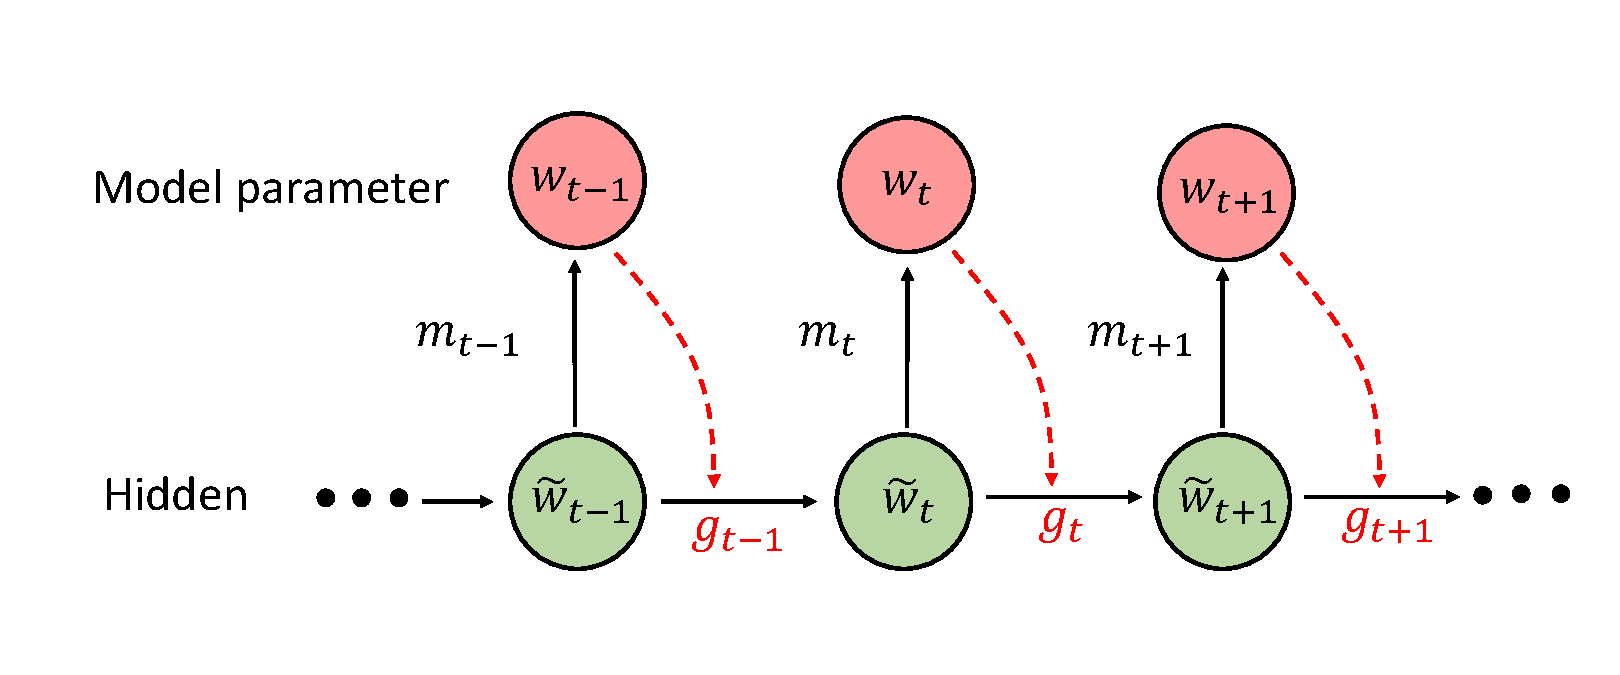
\includegraphics[width=2.7in]{plot.pdf}
    \caption{\textsc{OPT-AMSGRAD} Underlying Structure.}
     \label{fig:scheme}
\end{figure}
\end{minipage}

\vspace{-0.05in}
\section{Global Convergence Analysis of \textsc{OPT-AMSGrad}}\label{sec:analysis}
\vspace{-0.05in}


For conciseness, we place all the proofs of the following results in the supplementary material.\vspace{-0.05in}

\textbf{Notations.}\hspace{0.1in}
We denote the Mahalanobis norm $\|\cdot\|_H := \sqrt{ \langle \cdot, H \cdot \rangle }$ for some positive semidefinite (PSD) matrix $H$.
We let $\psi_t(x) := \langle x, \text{diag}\{\hat{v}_t\}^{1/2} x \rangle$ for a PSD matrix $H_t^{1/2}:= \text{diag}\{\hat{v}_t\}^{1/2}$, where $\text{diag}\{\hat{v}_t\}$ represents the diagonal matrix which $i_{th}$ diagonal element is $\hat{v}_t[i]$ defined in Algorithm~\ref{alg:optamsgrad}.
We define its corresponding Mahalanobis norm $\| \cdot \|_{\psi_t}:=  \sqrt{ \langle \cdot, \text{diag}\{\hat{v}_t\}^{1/2} \cdot \rangle }$,
where we abuse the notation $\psi_t$ to represent the PSD matrix $H_t^{1/2}:=\text{diag}\{\hat{v}_t\}^{1/2}$.
Note that $\psi_t(\cdot)$ is 1-strongly convex with respect to the norm $\| \cdot \|_{\psi_t}$.
Namely, $\psi_t(\cdot)$ satisfies $\psi_t(u) \geq \psi_t(v) + \langle \psi_t(v), u - v \rangle + \frac{1}{2} \| u - v\|^2_{\psi_t}$ for any point $(u,v) \in \Theta^2$.
A consequence of 1-strongly convexity of $\psi_t(\cdot)$ is that $B_{\psi_t}(u,v) \geq \frac{1}{2} \| u - v \|^2_{\psi_t}$, where the Bregman divergence $B_{\psi_t}(u,v)$ is defined as $B_{\psi_t}(u,v) := \psi_t(u) - \psi_t(v) - \langle \psi_t(v), u - v \rangle$ with $\psi_t(\cdot)$ as the distance generating function.
We also define the corresponding dual norm $\| \cdot \|_{\psi_t^*}:= \sqrt{ \langle \cdot, \text{diag}\{\hat{v}_t\}^{-1/2} \cdot \rangle }$.

\vspace{-0.05in}
\subsection{Convex Regret Analysis}
\vspace{-0.05in}

In this section, we assume that the loss functions $\{\ell_t\}_{t>0}$ are convex. 
We also assume that $\Theta$ has bounded diameter $D_{\infty}$, which is a standard assumption in previous works \citep{RKK18,KB15} on adaptive methods. It is necessary in regret analysis since if the boundedness assumption is lifted, one might construct a scenario such that the benchmark is $w^* = \infty$ and the learner's regret is infinite. 
\begin{Theorem} \label{thm:mainconvex}
Suppose the learner incurs a sequence of convex loss functions $\{ \ell_{t}(\cdot) \}$.
Then,  \textsc{OPT-AMSGrad} (Algorithm~\ref{alg:optamsgrad}) has regret 
\begin{equation} \notag
\begin{aligned}
\mathcal{R}_T \leq &   \frac{ B_{\psi_1}(w^*, \tilde{w}_{1})}{\eta_1}
+ \sum_{t=1}^T\frac{\eta_t}{2} \| g_t - \tilde{m}_t  \|_{\psi_{t-1}^*}^2  + \frac{D_{\infty}^2}{\eta_{\min}}  \sum_{i=1}^d \hat{v}_{T}^{1/2}[i] + D_{\infty}^2\beta_1^2   \sum_{t=1}^T  \| g_t - \theta_{t-1}  \|_{\psi_{t-1}^*}\eqsp,
\end{aligned}
\end{equation}
where $ \tilde{m}_{t+1}  = \beta_1 \theta_{t-1} +(1-\beta_1) m_{t+1}$, $g_{t}:= \nabla \ell_{t}(w_t)$, $\eta_{{\min}} := \min_{{t}} \eta_{t}$ and $D_{\infty}^2$ is the diameter of the bounded set $\Theta$.
The result holds for any benchmark $w^{*} \in \Theta$ and any step size sequence $\{ \eta_t \}_{t>0}$.
\end{Theorem}

\begin{Corollary}\label{cor:corollary}
Suppose $\beta_1=0$ and $\{v_t\}_{t>0}$ is a monotonically increasing sequence, then we obtain the following regret bound for any $w^{*} \in \Theta$ and sequence of stepsizes $\{ \eta_t = \eta/\sqrt{t}\}_{t>0}$: 
\begin{equation}\notag
\begin{aligned}
\mathcal{R}_T \leq & \frac{ B_{\psi_1}}{\eta_1}
+ \frac{\eta \sqrt{1 + \log T}}{\sqrt{1 - \beta_2}} \sum_{i=1}^d \| (g-m)_{1:T}[i] \|_2 +\frac{D_{\infty}^2}{\eta_{\min}} \sum_{i=1}^d \left[ (1-\beta_2) \sum_{s=1}^{T} \beta_2^{T-s} g^2_s[i] \right]^{1/2} \eqsp,
\end{aligned}
\end{equation}
where $B_{\psi_1} := B_{\psi_1}(w^*, \tilde{w}_{1})$, $g_{t}:= \nabla \ell_{t}(w_t)$ and $\eta_{{\min}} := \min_{{t}} \eta_{t}$.
\end{Corollary}
We can compare the bound of Corollary~\ref{cor:corollary} with that of \textsc{AMSGrad} \citep{RKK18} with $\eta_t = \eta/\sqrt{t}$:
\beq\label{eq:boundAMS}
\mathcal{R}_T \leq \frac{ \eta \sqrt{ 1 + \log T}    }{ \sqrt{1 - \beta_2}  } \sum_{i=1}^d \| g_{1:T}[i]  \|_2 +\frac{\sqrt{T}}{2 \eta} D^2_{\infty} \sum_{i=1}^d \hat{v}_T[i]^2 \eqsp.
\eeq
For convex regret minimization, the results above yields that the learner suffers regret of $\mathcal{O}(\sqrt{\sum_{t=1}^T \| g_t - m_t  \|^2_{\psi^*_{t-1}}})$ with an access to an arbitrary predictable process $\{m_t\}_{t>0}$ of the mini-batch gradients. 
The better the predictors, the lower the regret, which can be seen from the second term in Corollary~\ref{cor:corollary} compared to the first term in \eqref{eq:boundAMS}.
The construction of the predictable process $\{m_t\}_{t>0}$ is thus of utmost importance for achieving optimal acceleration and can be learned through the iterations.
We will not deal with the latter in this paper for the sake of space and clarity.
Though, for implementation purposes, we derive a simple, yet effective, gradient prediction algorithm, see Algorithm~\ref{alg:algex} in Section~\ref{sec:numerical}, embedded in our \textsc{OPT-AMSGrad} algorithm.

\vspace{-0.05in}
\subsection{Nonconvex Analysis (Finite-Time Upper Bound)}
\vspace{-0.05in}


We discuss the offline and stochastic nonconvex optimization properties of our online framework.
As stated in the Introduction, this paper is about solving optimization problems instead of solving zero-sum games.  
Classically, the problem we are tackling reads:
\beq\label{eq:minproblem}
\min \limits_{w \in \Theta} f(w) \eqdef  \EE[ f(w, \xi)] = n^{-1} \sum_{i=1}^n  \EE[f(w, \xi_i)] \eqsp,
\eeq
for a fixed batch of $n$ samples $\{ \xi_i \}_{i=1}^n$.
The objective function $f(w)$ is (potentially) nonconvex and has Lipschitz gradients.
Set the terminating number, $T \in \{0,\dots,T_{\sf M}-1\}$, as a discrete r.v.~with:
\beq \label{eq:random}
   P( T = \ell ) = \frac{ \eta_{\ell} }{\sum_{j=0}^{T_{\sf M}-1} \eta_j} \eqsp,
\eeq
where $T_{\sf M}$ is the maximum number of iteration.
The random termination number \eqref{eq:random} is inspired by \citep{ghadimi2013stochastic} and is widely used for nonconvex optimization. 
Assume the following:
%\begin{assumption}\label{ass:nonconv}
%The loss function $f(w)$ is nonconvex \wrt the parameter $w$.
%\end{assumption}
\begin{assumption}\label{ass:boundedparam}
For any $t >0$, the estimated weight $w_t$ stays within a $\ell_{\infty}-$ball. There exists a constant $W >0$ such that $\norm{w_t} \leq W$ almost surely.
\end{assumption}
\begin{assumption}\label{ass:smooth}
The function $f$ is $L$-smooth (has $L$-Lipschitz gradients) w.r.t. the parameter w.
There exists some constant $L > 0$ such that for $(w, \vartheta) \in \Theta^2$, $f(w) - f(\vartheta) - \nabla f(\vartheta)^\top(w - \vartheta) \leq \frac{L}{2} \norm{w - \vartheta}^2\eqsp.$
\end{assumption}
We assume that the optimistic guess $m_t$ at iteration $t$ and the true gradient $g_t$ are correlated:
\begin{assumption}\label{ass:guessbound}
There exists a constant $a \in \rset^* $ such that for any $t >0$, $ \pscal{m_t}{ g_t}  \leq a \|g_t\|^2$.
\end{assumption}
Classically in nonconvex optimization \citep{ghadimi2013stochastic} we make an assumption on the magnitude of the gradient:
\begin{assumption}\label{ass:bounded}
There exists a constant $\major >0$ such that for any $w$ and $\xi$, it holds $\norm{\nabla f(w, \xi)} < \major$.
\end{assumption}
We now derive important auxiliary Lemmas for our global analysis.
The first one ensures bounded norms of quantities of interests (resulting from the bounded stochastic gradient assumption):
\begin{Lemma}\label{lem:bound}
Assume H\ref{ass:bounded}, then the quantities defined in Algorithm~\ref{alg:optamsgrad} satisfy for any $w \in \Theta$ and $t>0$, $ \|\nabla f(w_t)\| < \major ,~~~\|\theta_t \| < \major$ and $\|\hat{v}_t\| < \major^2$.
\end{Lemma}
%Then, following \citep{yan2018unified} and their study of the SGD with Momentum we denote for any $t >0$:
%\beq\label{eq:deftilde}
%\overline{w}_t = w_t + \frac{\beta_1}{1 - \beta_1} (w_t - \tilde{w}_{t-1}) = \frac{1}{1 - \beta_1} w_t -  \frac{\beta_1}{1 - \beta_1} \tilde{w}_{t-1} \eqsp,
%\eeq
%\begin{Lemma}\label{lem:momentum}
%Assume a strictly positive and non increasing sequence of stepsizes $\{\eta_t \}_{t>0}$, $\beta_1 < \beta_2 \in [0,1)$, then the following holds:
%\beq\notag
%\overline{w}_{t+1} - \overline{w}_t \leq \frac{\beta_1}{1 - \beta_1} \tilde{\theta}_{t-1} \left[ \eta_{t-1} \hat{v}_{t-1}^{-1/2} - \eta_{t} \hat{v}_{t}^{-1/2}\right] - \eta_{t} \hat{v}_{t}^{-1/2} \tilde{g}_t \eqsp,
%\eeq
%where $\tilde{\theta}_t = \theta_t + \beta_1 \theta_{t-1}$ and $\tilde{g}_t = g_t - \beta_1 m_t + \beta_1 g_{t-1} + m_{t+1} $.
%\end{Lemma}
%\begin{Lemma}\label{lem:squarev}
%Assume H\ref{ass:bounded}, a strictly positive and a sequence of constant stepsizes $\{\eta_t \}_{t>0}$, $\beta_1 < \beta_2 \in [0,1)$, denote $\gamma = \beta_1/\beta_2$, then, 
%$\sum_{k=1}^{T_{\sf M}} \eta_{t}^{2} \EE [\|\hat{v}_{t}^{-1/2} \theta_{t} \|_{2}^{2}] \leq  \eta^{2} d T_{\sf M} (1- \beta_1)/[(1 - \beta_2)(1-\gamma)]$.
%\end{Lemma}
We now formulate the main result of our paper yielding a finite-time upper bound of the suboptimality condition $\EE\left[\|\nabla f(w_T)\|^2\right]$ (as the convergence criterion of interest, see \citep{ghadimi2013stochastic}):
\begin{Theorem}\label{thm:boundopt}
Assume H\ref{ass:boundedparam}-H\ref{ass:bounded}, $\beta_1 < \beta_2 \in [0,1)$ and a sequence of decreasing stepsizes $\{\eta_t\}_{t>0}$, then the following result holds:
\beq\notag
\begin{split}
\EE\left[\|\nabla f(w_T)\|^2\right] \leq \tilde{C}_1 \sqrt{\frac{d}{T_{\sf M}}} + \tilde{C}_2 \frac{1}{T_{\sf M}} \eqsp,
\end{split}
\eeq
where $T$ is a random termination number distributed according \eqref{eq:random}.
The constants are defined as:
\begin{align*}
&\tilde{C}_1 = C_1 +  \frac{\major}{(1 - a\beta_1) + (\beta_1 + a)} \left[ \frac{a(1 - \beta_1)^2}{1-\beta_2} + 2L \frac{1}{1-\beta_2} +  \Delta f  +   \frac{4L \beta_1^2(1 + \beta_1^2) }{(1 - \beta_1)(1 - \beta_2)(1-\gamma)} \right]\\
&\tilde{C}_2 = \frac{ (a\beta_1^2 -2 a \beta_1 + \beta 1)\major^2 }{(1 - \beta_1) \left((1 - a\beta_1) + (\beta_1 + a)\right)}  \EE\left[ \norm{\hat{v}_{0}^{-1/2}}    \right]  \quad \textrm{where} \quad \Delta f = f(\overline{w}_{1}) - f(\overline{w}_{T_{\sf M}+1})
\end{align*}
\end{Theorem}
We remark that the bound for our OPT-AMSGrad method matches the complexity bound of $\mathcal{O}\left( \sqrt{d/T_{\sf M}} + 1/T_{\sf M} \right)$ of \citep{ghadimi2013stochastic} for SGD and \citep{zhou2018convergence} for AMSGrad method.


\vspace{-0.05in}
\subsection{Checking H\ref{ass:boundedparam} for a Deep Neural Network}
\vspace{-0.05in}


As boundedness assumption H\ref{ass:boundedparam} is generally hard to verify, we now show, for illustrative purposes, that the weights of a fully connected feed forward neural network stay in a bounded set when being trained using our method. 
The activation function for this section will be sigmoid function and we use a $\ell_2$ regularization. 
We consider a fully connected feed forward neural network with $L$ layers modeled by the function $\textsf{MLN}(w, \xi): \Theta^d \times \rset^p \to \rset$:
\beq\label{eq:dnnmodel}
\textsf{MLN}( w, \xi) = \sigma\left(w^{(L)} \sigma\left(w^{(L-1)} \ldots \sigma\left(w^{(1)} \xi \right)\right)\right)
\eeq
where $w = [w^{(1)}, w^{(2)}, \cdots , w^{(L)}]$ is the vector of parameters, $\xi \in \rset^p$ is the input data and $\sigma$ is the sigmoid activation function. We assume a $p$ dimension input data and a scalar output for simplicity.
The stochastic objective function \eqref{eq:minproblem} reads:
\beq \notag
f(w, \xi) = \mathcal{L}(\textsf{MLN}( w, \xi), y) +\frac{\lambda}{2}\norm{w}^2
\eeq
where $\mathcal{L}(\cdot, y)$ is the loss function (can be Huber loss or cross entropy), $y$ are the true labels and $\lambda >0$ is the regularization parameter.
For any index $\ell \in [1, L]$ we denote the output of layer $\ell$ by 
$$
h^{(\ell)}(w,\xi)= \sigma\left(w^{(\ell)} \sigma\left(w^{(\ell-1)} \ldots \sigma\left(w^{(1)} \xi \right)\right)\right) \eqsp.
$$
The following Lemma proves that assumption H\ref{ass:boundedparam} is satisfied with a feed forward neural net \eqref{eq:dnnmodel}:
\begin{Lemma}\label{lem:dnnh2} 
Given the multilayer model \eqref{eq:dnnmodel}, assume the boundedness of the input data and of the loss function, \ie for any $\xi \in \rset^p$ and $y \in \rset$ there is a constant $T >0$ such that $\norm{\xi} \leq 1 \quad \textrm{a.s.}$ and $|\mathcal{L}'(\cdot, y)| \leq T$ where $\mathcal{L}'(\cdot, y)$ denotes its derivative \wrt the parameter. Then for each layer $\ell \in [1,L]$, there exist a constant $A_{(\ell)}$ such that $\norm{w^{(\ell)}} \leq A_{(\ell)}$
\end{Lemma}

\vspace{-0.05in}
\section{Numerical Experiments}\label{sec:numerical}
\vspace{-0.05in}

\subsection{Gradient Estimation}
\vspace{-0.05in}

From the analysis in the previous section, we understand that the choice of the prediction $m_t$ plays an important role in the convergence of \textsc{Optimistic-AMSGrad}.
%In \textsc{Optimistic-Online learning}, $m_{t}$ is usually set to $m_{t}= g_{t-1}$, which means that it uses the previous gradient as a guess of the next one.
%The choice can accelerate the convergence to equilibrium in some two-player zero-sum games \cite{RS13,SALS15,DISZ18}, in which each player uses an optimistic online learning algorithm against its opponent.
%We propose to use the extrapolation algorithm of \citep{SAB16} based on estimating the limit of a sequence using the last iterates \citep{BZ13}. 
Some classical works in gradient prediction methods include \textsc{Anderson} acceleration \citep{WN11}, \textsc{Minimal Polynomial Extrapolation} \citep{CJ76},  \textsc{Reduced Rank Extrapolation} \citep{E79}.
%These methods assume that the sequence $\{g_t\} \in \mathbb R^d$ has a linear relation $g_t = A( g_{t-1} - g^* ) + g^*$ where $A \in \mathbb R^{d \times d}$ is unknown and finds the fixed point $g^{*}$. 
%\citep{SAB16} relaxes the assumption to certain degrees. 
These methods aim at finding a fixed point $g^{*}$ and assume that $\{g_t \in \mathbb R^d\}_{t>0} $ has the following linear relation:\vspace{-0.1cm}
\begin{equation} \label{nox}
g_t - g^* = A( g_{t-1} - g^* ) + e_t,
\end{equation}
where $e_t$ is a second order term satisfying $\| e_t \|_2  = \mathcal{O}( \| g_{t-1} - g^* \|_2^2)$ and $A \in \mathbb R^{d \times d}$ is an unknown matrix, see \citep{SAB16} for details and results.
For our numerical experiments, we run \textsc{OPT-AMSGrad} using Algorithm~\ref{alg:algex} to construct the sequence $\{m_t\}_{t>0}$ and based on estimating the limit of a sequence using the last iterates \citep{BZ13}.
\begin{algorithm}[H]
\begin{algorithmic}[1] 
\small
\caption{\textsc{Regularized Approximate Minimal Polynomial Extrapolation}
\citep{SAB16} } \label{alg:algex}
\STATE \textbf{Input:} sequence $\{ g_s \in \mathbb R^d \}_{s=0}^{s=r-1}$, parameter $\lambda > 0$.
\STATE Compute matrix  $U = [ g_1 - g_0, \dots, g_{r} - g_{r-1}] \in \mathbb R^{d \times r}$.
\STATE Obtain $z$ by solving $(U^\top U + \lambda I ) z = \mathbf{1}$.
\STATE Get $c= z / (z^\top \mathbf{1})$.
\STATE \textbf{Output:} $\Sigma_{i=0}^{r-1} c_i g_i$, the approximation of the fixed point $g^*$.
\end{algorithmic}
\end{algorithm}\vspace{-0.1in}
Specifically, at iteration $t$, $m_t$ is obtained by \textsf{(a)} calling Algorithm~\ref{alg:algex} with a sequence of past $r$ gradients, $\{ g_{t-1},g_{t-2}, \dots, g_{t-r} \}$ as input and \textsf{(b)} setting $m_t:= \Sigma_{i=0}^{r-1} c_i g_{t-r+i}$ where $c = [c_0, \dots, c_{r-1}] $ is obtained by Algorithm~\ref{alg:algex}.
To see why the output from the extrapolation method may be a reasonable estimation, assume that the update converges to a stationary point (i.e. $g^*:=\nabla f(w^*) = 0$ for the underlying function $f$). Then, we might rewrite (\ref{nox}) as $g_t = A g_{t-1}  + \mathcal{O}( \| g_{t-1} \|_2^2 ) u_{t-1}$, for some unit vector $u_{t-1}$.
This equation suggests that the next gradient vector $g_{t}$ is a linear transform of $g_{{t-1}}$ plus an error vector that may not be in the span of $A$.
If the algorithm is converges to a stationary point, the magnitude of the error will converge to zero.

\textbf{Computational cost:}
 This extrapolation step consists in: \textsf{(a)} Constructing the linear system $(U^\top U)$ which cost can be optimized to $\mathcal{O}(d)$, since the matrix $U$ only changes one column at a time. \textsf{(b)} Solving the linear system which cost is $\mathcal{O}(r^3)$, and is negligible for a small $r$ used in practice.\textsf{ (c)} Outputting a weighted average of previous gradients which cost is $\mathcal{O}(r \times d)$ yielding a computational overhead of $\mathcal O\left((r+1)d+r^3\right)$.
Yet, steps (a) and (c) are parallelizable in the final implementation.

\vspace{-0.05in}
\subsection{Classification Experiments}
\vspace{-0.05in}

In this section, we provide experiments on classification tasks with various neural network architectures and datasets to demonstrate the effectiveness of \textsc{OPT-AMSGrad}.

\textbf{Methods.}
We consider two baselines. The first one is the original \textsc{AMSGrad}. 
The hyper-parameters are set to be $\beta_1 = 0.9$ and $\beta_2 = 0.999$, see \citep{RKK18}. 
The other benchmark method is the \textsc{Optimistic-Adam$+\hat{v}_t$} \citep{DISZ18}, which details are reported to the supplementary material. 
We use cross-entropy loss, a mini-batch size of $128$ and tune the learning rates over a fine grid and report the best result for all methods.
For \textsc{OPT-AMSGrad}, we use $\beta_1 = 0.9$ and $\beta_2 = 0.999$ and the best step size $\eta$ of \textsc{AMSGrad} for a fair evaluation of the optimistic step. 
\textsc{OPT-AMSGrad} has an additional parameter $r$ that controls the number of previous gradients used for gradient prediction. 
%Fortunately, we observe similar performance of \textsc{OPT-AMSGrad} with different values of $r$. 
%Hence, we report the result of $r=5$. Comparison among different $r$ can be found in the Supplemental Material.
%In the sequel, we use $r=5$ past gradient for empirical reasons, see Section~\ref{sec:choicer}.
We use $r=5$ past gradient for empirical reasons, see Section~\ref{sec:choicer}.
The algorithms are initialized at the same point and the results are averaged over 5 repetitions.

\textbf{Datasets.}
We compare different algorithms on \textit{MNIST}, \textit{CIFAR10},
\textit{CIFAR100}, and \textit{IMDB} datasets. 
For \textit{MNIST}, we use two noisy variants called \textit{MNIST-back-rand} and \textit{MNIST-back-image} from \citep{MNIST07} ($n=12\,000$), \textit{CIFAR10} and \textit{CIFAR100} \citep{krizhevsky2009learning} ($n=50\,000$) and \textit{IMDB} \citep{IMDB11} ($n=25\,000$). 
%They both have 12000 training samples and 50000 test samples, where random background is inserted to the original \textit{MNIST} hand written digit images. 
% For \textit{MNIST-back-rand}, each image is inserted with a random background, whose pixel values generated uniformly from 0 to 255, while \textit{MNIST-back-image} takes random patches from a black and white as noisy background.
%The input dimension is 784 ($28\times 28$) and the number of classes is $10$.
% \textit{CIFAR10} and \textit{CIFAR100} are popular computer-vision datasets consisting of 50000 training images and 10000 test images, of size $32\times 32$. 
% The number of classes are 10 and 100, respectively. 
% The \textit{IMDB} movie review dataset is a binary classification dataset with 25000 training and testing samples respectively. It is a popular datasets for text classification.

\textbf{Network architecture.} We adopt a multi-layer fully connected neural network with hidden layers of $200$ then $100$ neurons (using \textrm{ReLU} activations and \textrm{Softmax} output) on \textit{MNIST} variants. 
For CIFAR datasets, we adopt ALL-CNN network proposed by \citep{CNN15}, built with convolutional blocks and dropout layers.
 In addition, we also apply residual networks, Resnet-18 and Resnet-50~\citep{Rnet16}, which have achieved state-of-the-art results.
For the texture \textit{IMDB} dataset, we consider a Long-Short Term Memory (LSTM) network \citep{gers1999learning} including a word embedding layer with $5\,000$ input entries representing most frequent words embedded into a $32$ dimensional space. 
The output of the embedding layer is passed to $100$ LSTM units then connected to $100$ fully connected \textrm{ReLU} layers. \vspace{-0.1in}


\begin{figure}[H]
\centering
\mbox{\hspace{-0.2in}
\includegraphics[width=1.8in]{simulation/fig2/M_rand_train_loss_no1.eps}\hspace{-0.1in}
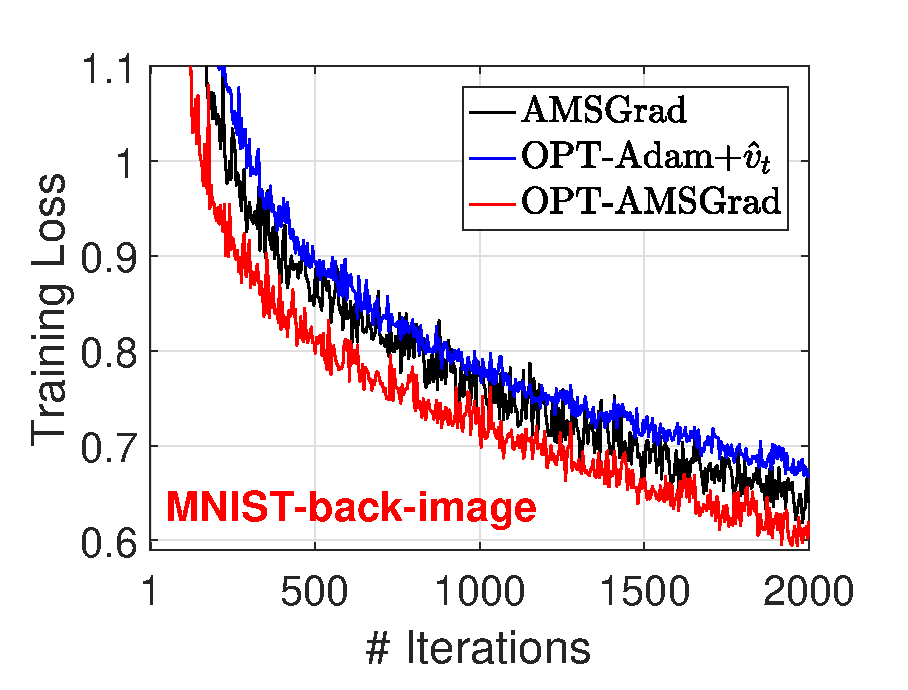
\includegraphics[width=1.8in]{simulation/fig2/M_image_train_loss_no1.eps}\hspace{-0.1in}
\includegraphics[width=1.8in]{simulation/fig2/cifar_cnn_train_loss_no1.eps}
}

\mbox{\hspace{-0.2in}
\includegraphics[width=1.8in]{simulation/fig2/imdb_lstm_train_loss_no1.eps}\hspace{-0.1in}
\includegraphics[width=1.8in]{simulation/fig2/cifar10_resnet_train_loss.eps}\hspace{-0.1in}
\includegraphics[width=1.8in]{simulation/fig2/cifar100_resnet_train_loss.eps}
}
\caption{Training loss vs. Number of iterations for fully connected NN, LSTM, CNN and ResNet.}
\label{fig:train_loss}\vspace{-0.15in}
\end{figure}

\textbf{Results.} 
Firstly, to illustrate the acceleration effect of \textsc{OPT-AMSGrad} at early stage, we provide the training loss against number of iterations in Figure~\ref{fig:train_loss}. 
We clearly observe that on all datasets, the proposed \textsc{OPT-AMSGrad} converges faster than the other competing methods since fewer iterations are required to achieve the same precision validating one of the main edges of \textsc{OPT-AMSGrad}.
We are also curious about the long-term performance and generalization of the proposed method in test phase.
In Figure~\ref{fig:testandtrain}, we plot the results when the model is trained until the test accuracy stabilizes. 
We observe: \textsf{(1)} in the long term, \textsc{OPT-AMSGrad} algorithm may converge to a better point with smaller objective function value, and \textsf{(2)} in these three applications, the proposed \textsc{OPT-AMSGrad} also outperforms the competing methods in terms of test accuracy. \vspace{-0.1in}

\begin{figure}[H]
\mbox{\hspace{-0.2in}
\includegraphics[width=1.5in]{new_figure/new_mnist_img_figure/mnist_img_train_loss_disz_2.eps}\hspace{-0.12in}
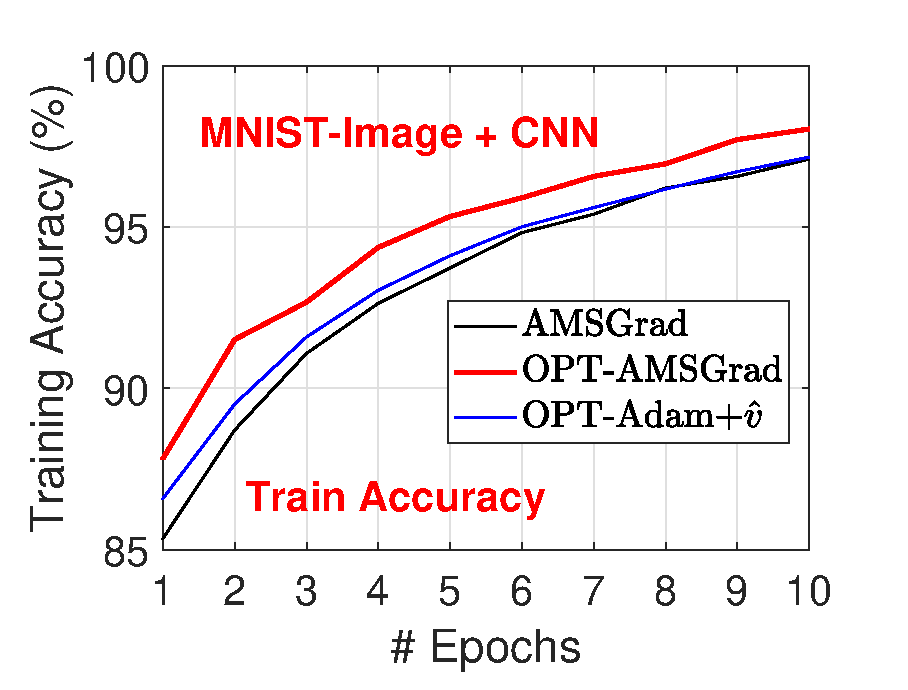
\includegraphics[width=1.5in]{new_figure/new_mnist_img_figure/mnist_img_train_acc_disz_2.eps}\hspace{-0.12in}
\includegraphics[width=1.5in]{new_figure/mnist_img_test_loss_disz.eps}\hspace{-0.12in}
\includegraphics[width=1.5in]{new_figure/mnist_img_test_acc_disz.eps}
}

\mbox{\hspace{-0.2in}
\includegraphics[width=1.5in]{new_figure/cifar10_train_loss_disz.eps}\hspace{-0.12in}
\includegraphics[width=1.5in]{new_figure/cifar10_train_acc_disz.eps}\hspace{-0.12in}
\includegraphics[width=1.5in]{new_figure/cifar10_test_loss_disz.eps}\hspace{-0.12in}
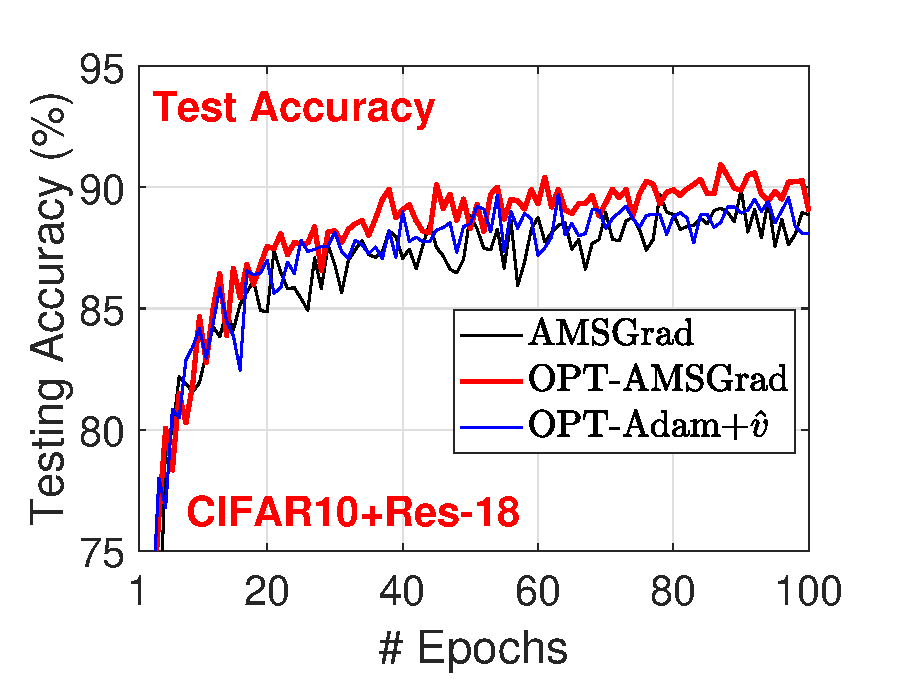
\includegraphics[width=1.5in]{new_figure/cifar10_test_acc_disz.eps}
}

\mbox{\hspace{-0.2in}
\includegraphics[width=1.5in]{new_figure/cifar100_train_loss_disz.eps}\hspace{-0.12in}
\includegraphics[width=1.5in]{new_figure/cifar100_train_acc_disz.eps}\hspace{-0.12in}
\includegraphics[width=1.5in]{new_figure/cifar100_train_loss_disz.eps}\hspace{-0.12in}
\includegraphics[width=1.5in]{new_figure/cifar100_test_acc_disz.eps}
}
\vspace{-0.15in}
\caption{\textit{MNIST-back-image} + CNN, \textit{CIFAR10} + Res-18 and \textit{CIFAR100} + Res-50 . We compare three methods in terms of training (cross-entropy) loss and accuracy, testing loss and accuracy.} \label{fig:testandtrain}\vspace{-0.15in}
\end{figure}

\vspace{-0.05in}
\subsection{Choice of parameter $r$}\label{sec:choicer}
\vspace{-0.05in}


\begin{wrapfigure}{r}{3in}\vspace{-0.3in}
\begin{center}
\mbox{
\includegraphics[width=1.5in]{new_figure/new_mnist_img_figure/mnist_img_train_loss_r3510_2.eps}\hspace{-0.1in}
\includegraphics[width=1.5in]{new_figure/cifar10_train_loss_r3510.eps}
}
\end{center}
\caption{Training loss w.r.t. $r$.}\label{fig:compare}\vspace{-0.1in}
\end{wrapfigure}

Since the number of past gradients $r$ is important in our algorithm, we compare Figure~\ref{fig:compare} the performance under different values $r=3,5,10$ on two datasets. 
From the result we see that the choice of $r$ does not have significant impact on the training loss.
Taking into consideration both quality of gradient prediction and computational cost, $r=5$ is a good choice for most applications here. 
We remark that empirically, the performance comparison among $r=3,5,10$ is not absolutely consistent (i.e. more means better) in all cases. 
One possible reason is that for deep neural networks, the high diversity of gradients computed through the iterations, due to the nonconvexity of the loss, makes most of them inefficient for the predictable process $\{m_t\}_{t>0}$. Only recent ones ($r \leq 5$) are useful.\vspace{-0.1in}

\vspace{-0.05in}
\section{Conclusion}
\vspace{-0.1in}

In this paper, we propose \textsc{OPT-AMSGrad}, which combines optimistic online learning and \textsc{AMSGrad} to improve sample efficiency and
accelerate the process of training, in particular for deep neural networks. 
Given a good gradient prediction process, we demonstrate that the regret can be smaller than that of standard \textsc{AMSGrad}.
We also establish finite-time convergence bound on the second order moment of the gradient of the objective function matching that of state-of-the-art algorithms.
Experiments on various deep learning problems demonstrate the effectiveness of the proposed method in accelerating the empirical risk minimization procedure and empirically show better generalization properties of our method.


\clearpage

\bibliographystyle{abbrvnat}
\bibliography{reference}

\clearpage


\appendix


\section{Proof of Theorem~\ref{thm:mainconvex}}\label{app:thmmainconvex}
\begin{Theorem*}
Suppose the learner incurs a sequence of convex loss functions $\{ \ell_{t}(\cdot) \}$.
Then,  \textsc{OPT-AMSGrad} (Algorithm~\ref{alg:optamsgrad}) has regret 
\begin{equation}\notag
\begin{aligned}
\mathcal{R}_T \leq &   \frac{ B_{\psi_1}(w^*, \tilde{w}_{1})}{\eta_1}
+ \sum_{t=1}^T\frac{\eta_t}{2} \| g_t - \tilde{m}_t  \|_{\psi_{t-1}^*}^2  + \frac{D_{\infty}^2}{\eta_{\min}}  \sum_{i=1}^d \hat{v}_{T}^{1/2}[i] + D_{\infty}^2\beta_1^2   \sum_{t=1}^T  \| g_t - \theta_{t-1}  \|_{\psi_{t-1}^*}\eqsp,
\end{aligned}
\end{equation}
where $ \tilde{m}_{t+1}  = \beta_1 \theta_{t-1} +(1-\beta_1) m_{t+1}$, $g_{t}:= \nabla \ell_{t}(w_t)$, $\eta_{{\min}} := \min_{{t}} \eta_{t}$ and $D_{\infty}^2$ is the diameter of the bounded set $\Theta$.
The result holds for any benchmark $w^{*} \in \Theta$ and any step size sequence $\{ \eta_t \}_{t>0}$.
\end{Theorem*}

\begin{proof}
Beforehand, note:
\beq
\begin{split}
& \tilde{g}_t  = \beta_1 \theta_{t-1} +(1 - \beta_1) g_t\\
& \tilde{m}_{t+1}  = \beta_1 \theta_{t-1} +(1-\beta_1) m_{t+1}
\end{split}
\eeq
where we recall that $g_t$ and $m_{t+1}$ are respectively the gradient $\nabla \ell_t(w_t)$ and the predictable guess.
By regret decomposition, we have that
\begin{equation} \label{nn1}
\begin{aligned}
 &\text{\it Regret}_T := \sum_{t=1}^T \ell_t(w_t) - \min_{w \in \Theta} \sum_{t=1}^T \ell_t(w)  \textstyle  \\
  \leq & \sum_{t=1}^T  \langle w_t - w^*, \nabla \ell_t(w_t) \rangle
\\  = &\sum_{t=1}^T \langle  w_t - \tilde{w}_{t+1} , g_t - \tilde{m}_t \rangle + \langle w_t - \tilde{w}_{t+1}, \tilde{m}_t \rangle + \langle \tilde{w}_{t+1} - w^*, \tilde{g}_t  \rangle+ \langle \tilde{w}_{t+1} - w^*,g_t - \tilde{g}_t  \rangle \eqsp.
\end{aligned}
\end{equation}

Recall the notation $\psi_t(x)$ and the Bregman divergence $B_{\psi_t}(u,v)$
we defined in the beginning of this section.
Now we are going to exploit a useful inequality (which appears in e.g.,~\citep{T08}); for any update of the form $\hat{w} = \arg\min_{w \in \Theta} \langle w, \theta \rangle + B_{\psi}(w, v)$, it holds that
\begin{equation} \label{ii}
\langle \hat{w} - u, \theta \rangle \leq B_{\psi}( u, v ) - B_{\psi}( u, \hat{w}) - B_{\psi}( \hat{w}, v) \quad \textrm{for any $u \in \Theta$} \eqsp.
\end{equation}
For $\beta_1=0$, we can rewrite the update on line 8 of (Algorithm~\ref{alg:optamsgrad}) as
\begin{equation} \label{nc1}
\tilde{w}_{t+1}= \arg\min_{w \in \Theta} \eta_t \langle w, \tilde{g}_t \rangle + B_{\psi_t}(w, \tilde{w}_{t} ) \eqsp,
\end{equation}
By using (\ref{ii}) for (\ref{nc1}) with $\hat{w} = \tilde{w}_{t+1}$ (the output of the minimization problem), $u = w^*$ and $v = \tilde{w}_{t}$, we have
\begin{equation} \label{nn2}
\begin{aligned}
 \langle \tilde{w}_{t+1} - w^*, & \tilde{g}_t \rangle \leq \frac{1}{\eta_t}\big[ B_{\psi_t}( w^*, \tilde{w}_{t}) -B_{\psi_t}(w^*,  \tilde{w}_{t+1} ) - B_{\psi_t}(\tilde{w}_{t+1}, \tilde{w}_{t}) \big] \eqsp.
\end{aligned}
\end{equation}

We can also rewrite the update on line 9 of (Algorithm~\ref{alg:optamsgrad}) at time $t$ as
\begin{equation} \label{nc2}
\textstyle w_{t+1} = \arg\min_{w \in \Theta} \eta_{t+1} \langle w, \tilde{m}_{t+1} \rangle + B_{\psi_t}(w, \tilde{w}_{t+1} ).
\end{equation}
and, by using \eqref{ii} for \eqref{nc2} (written at iteration $t$), with $\hat{w} = w_{t}$ (the output of the minimization problem), $u = \tilde{w}_{t+1}$ and $v = \tilde{w}_{t}$, we have
\begin{equation} \label{nn3}
\begin{aligned}
\langle w_t -\tilde{w}_{t+1}, & \tilde{m}_t  \rangle \leq \frac{1}{\eta_t}\big[ B_{\psi_{t-1}}(\tilde{w}_{t+1}, \tilde{w}_{t}) - B_{\psi_{t-1}}(\tilde{w}_{t+1}, w_t ) - B_{\psi_{t-1}}(w_{t}, \tilde{w}_{t}) \big] \eqsp,
\end{aligned}
\end{equation}
By (\ref{nn1}), (\ref{nn2}), and (\ref{nn3}), we obtain
\begin{equation} \label{nnn}
\begin{aligned}
 \mathcal{R}_T & \overset{(\ref{nn1})}{\leq} \sum_{t=1}^T \langle  w_t - \tilde{w}_{t+1} , g_t - \tilde{m}_t \rangle + \langle w_t - \tilde{w}_{t+1}, \tilde{m}_t \rangle + \langle \tilde{w}_{t+1} - w^*, \tilde{g}_t  \rangle+ \langle \tilde{w}_{t+1} - w^*,g_t - \tilde{g}_t  \rangle \\
& \overset{(\ref{nn2}), (\ref{nn3})}{\leq}  \sum_{t=1}^T \| w_t - \tilde{w}_{t+1} \|_{\psi_{t-1}} \| g_t - \tilde{m}_t  \|_{\psi_{t-1}^*} + \|  \tilde{w}_{t+1} - w^* \|_{\psi_{t-1}} \| g_t - \tilde{g}_t  \|_{\psi_{t-1}^*}\\
&+ \frac{1}{\eta_t} \big[ B_{\psi_{t-1}}(\tilde{w}_{t+1}, \tilde{w}_{t}) - B_{\psi_{t-1}}(\tilde{w}_{t+1}, w_t ) - B_{\psi_{t-1}}(w_{t}, \tilde{w}_{t}) \\
& +  B_{\psi_t}( w^*, \tilde{w}_{t}) -B_{\psi_t}(w^*,  \tilde{w}_{t+1} ) - B_{\psi_t}(\tilde{w}_{t+1}, \tilde{w}_{t}) \big],
\end{aligned}
\end{equation}
which is further bounded by
\begin{equation} \label{nnnn}
\begin{aligned}
  \mathcal{R}_T \leq \sum_{t=1}^T \Big\{  & \frac{1}{2 \eta_t} \| w_t - \tilde{w}_{t+1} \|_{\psi_{t-1}}^2 + \frac{\eta_t}{2} \| g_t - m_t  \|_{\psi_{t-1}^*}^2+ \|  \tilde{w}_{t+1} - w^* \|_{\psi_{t-1}} \| g_t - \tilde{g}_t  \|_{\psi_{t-1}^*}\\\
 &  + \frac{1}{\eta_t} \big(\underbrace{B_{\psi_{t-1}}(\tilde{w}_{t+1}, \tilde{w}_{t}) - B_{\psi_t}(\tilde{w}_{t+1}, \tilde{w}_{t}) }_{A_1}- \frac{1}{2} \| \tilde{w}_{t+1} - w_t \|_{\psi_{t-1}}^2\\
 &+\underbrace{B_{\psi_t}( w^*, \tilde{w}_{t}) -B_{\psi_t}(w^*,  \tilde{w}_{t+1} )}_{A_2}  \big) \Big\} \eqsp,
\end{aligned}
\end{equation}
where the inequality is due to $ \| w_t - \tilde{w}_{t+1}   \|_{\psi_{t-1}} \| g_t - m_t  \|_{\psi_{t-1}^*} = \inf_{ \beta > 0 }   \frac{1}{2\beta} \| w_t - \tilde{w}_{t+1} \|_{\psi_{t-1}}^2 +  \frac{\beta}{2} \| g_t - m_t  \|_{\psi_{t-1}^*}^2$ by Young's inequality and the 1-strongly convex of $\psi_{t-1}(\cdot)$ with respect to $\| \cdot \|_{\psi_{t-1}}$ which yields that $B_{\psi_{t-1}}(\tilde{w}_{t+1}, w_t )  \geq \frac{1}{2} \| \tilde{w}_{t+1} -  w_t  \|^2_{\psi_t} \geq 0$. 

To proceed, notice that
\begin{equation} \label{nn5}
\begin{aligned}
A_1 =  B_{\psi_{t-1}}(\tilde{w}_{t+1}, \tilde{w}_{t}) - B_{\psi_t}(\tilde{w}_{t+1}, \tilde{w}_{t})  = \langle \tilde{w}_{t+1} - \tilde{w}_{t} , \text{diag}(\hat{v}_{t-1}^{1/2} -\hat{v}_t^{1/2} ) ( \tilde{w}_{t+1}- \tilde{w}_{t} ) \rangle \leq 0 \eqsp,
\end{aligned}
\end{equation}
as the sequence $\{\hat{v}_t\}$ is non-decreasing. And that
\begin{equation}  \label{nn4}
\begin{aligned}
A_2 = B_{\psi_t}( w^*, \tilde{w}_{t}) -B_{\psi_t}(w^*,  \tilde{w}_{t+1} )  &= \langle w^* - \tilde{w}_{t+1}  , \text{diag}(\hat{v}_{t+1}^{1/2} -\hat{v}_t^{1/2} ) ( w^* - \tilde{w}_{t+1}  ) \rangle\\
  & \leq ( \max_i (w^*[i] -  \tilde{w}_{t+1} [i] )^2  )\cdot ( \sum_{i=1}^d \hat{v}_{t+1}^{1/2}[i] -\hat{v}_t^{1/2}[i] )
\end{aligned}
\end{equation}
Therefore, by (\ref{nnnn}),(\ref{nn4}),(\ref{nn5}), we have
\begin{equation}\notag
\begin{aligned}
\mathcal{R}_T \leq & \frac{D_{\infty}^2}{\eta_{\min}}  \sum_{i=1}^d \hat{v}_{T}^{1/2}[i] + \frac{ B_{\psi_1}(w^*, \tilde{w}_{1})}{\eta_1}
+ \sum_{t=1}^T\frac{\eta_t}{2} \| g_t - \tilde{m}_t  \|_{\psi_{t-1}^*}^2  \\
& +D_{\infty}^2 \beta_1^2  \sum_{t=1}^T \| g_t - \theta_{t-1}  \|_{\psi_{t-1}^*}  \eqsp.
\end{aligned}
\end{equation}
since $  \| g_t - \tilde{g}_t  \|_{\psi_{t-1}^*} =  \| g_t - \beta_1 \theta_{t-1} -(1- \beta_1) g_t \|_{\psi_{t-1}^*} = \beta^2 \| g_t - \theta_{t-1}  \|_{\psi_{t-1}^*} $.
This completes the proof.

\end{proof}

\section{Proof of Corollary~\ref{cor:corollary}}
\begin{Corollary*}
Suppose $\beta_1=0$ and $\{v_t\}_{t>0}$ is a monotonically increasing sequence, then we obtain the following regret bound for any $w^{*} \in \Theta$ and sequence of stepsizes $\{ \eta_t = \eta/\sqrt{t}\}_{t>0}$: 
\begin{equation}\notag
\begin{aligned}
\mathcal{R}_T \leq & \frac{ B_{\psi_1}}{\eta_1}
+ \frac{\eta \sqrt{1 + \log T}}{\sqrt{1 - \beta_2}} \sum_{i=1}^d \| (g-m)_{1:T}[i] \|_2 +\frac{D_{\infty}^2}{\eta_{\min}} \sum_{i=1}^d \left[ (1-\beta_2) \sum_{s=1}^{T} \beta_2^{T-s} g^2_s[i] \right]^{1/2} \eqsp,
\end{aligned}
\end{equation}
where $B_{\psi_1} := B_{\psi_1}(w^*, \tilde{w}_{1})$, $g_{t}:= \nabla \ell_{t}(w_t)$ and $\eta_{{\min}} := \min_{{t}} \eta_{t}$.
\end{Corollary*}

\begin{proof}
Recall the bound in Theorem~\ref{thm:mainconvex}:
\begin{equation}\notag
\begin{aligned}
\mathcal{R}_T \leq &   \frac{ B_{\psi_1}(w^*, \tilde{w}_{1})}{\eta_1}
+ \sum_{t=1}^T\frac{\eta_t}{2} \| g_t - \tilde{m}_t  \|_{\psi_{t-1}^*}^2  + \frac{D_{\infty}^2}{\eta_{\min}}  \sum_{i=1}^d \hat{v}_{T}^{1/2}[i] + D_{\infty}^2\beta_1^2   \sum_{t=1}^T  \| g_t - \theta_{t-1}  \|_{\psi_{t-1}^*}\eqsp,
\end{aligned}
\end{equation}

The second term reads:
\begin{align*}
     &\sum_{t=1}^T \frac{\eta_t}{2} \|g_t - m_t  \|_{\psi_{t-1}^*}^2 \\
      =&\sum_{t=1}^{T-1} \frac{\eta_t}{2} \|g_t - m_t  \|_{\psi_{t-1}^*}^2   + \eta_T \sum_{i=1}^d \frac{ (g_{T}[i] - m_{T}[i])^2 }{ \sqrt{ v_{T-1}[i]} }\\
=&\sum_{t=1}^{T-1} \frac{\eta_t}{2} \|g_t - m_t  \|_{\psi_{t-1}^*}^2 + \eta \sum_{i=1}^d \frac{ (g_{T}[i] - m_{T}[i])^2 }{ \sqrt{ T \big( (1-\beta_2) \sum_{s=1}^{T-1} \beta_2^{T-1-s} (g_{s}[i] - m_{s}[i])^2 } \big) }\\
\leq &  \eta \sum_{i=1}^d \sum_{t=1}^T \frac{ (g_{t}[i] - m_{t}[i])^2 }{ \sqrt{ t \big( (1-\beta_2) \sum_{s=1}^{t-1} \beta_2^{t-1-s} (g_{s}[i] - m_{s}[i])^2 } \big) }.
\end{align*}
To interpret the bound, let us make a rough approximation such that
$\sum_{s=1}^{t-1} \beta_2^{t-1-s} (g_{s}[i] - m_{s}[i])^2  \simeq (g_{t}[i] - m_t[i])^2 $.
Then, we can further get an upper-bound as 
\begin{align*}
    \sum_{t=1}^T \frac{\eta_t}{2} \|g_t - m_t  \|_{\psi_{t-1}^*}^2 \leq
    \frac{\eta}{\sqrt{1 - \beta_2}} \sum_{i=1}^d \sum_{t=1}^{T} \frac{ | g_{t}[i] - m_{t}[i] | }{ \sqrt{t} }\leq \frac{\eta \sqrt{1 + \log T}}{\sqrt{1 - \beta_2}} \sum_{i=1}^d \| (g-m)_{1:T}[i] \|_2 ,
\end{align*}
where the last inequality is due to Cauchy-Schwarz.


\end{proof}

\clearpage
\section{Proofs of Auxiliary Lemmas}
Following \citep{yan2018unified} and their study of the SGD with Momentum we denote for any $t >0$:
\beq\label{eq:deftilde}
\overline{w}_t = w_t + \frac{\beta_1}{1 - \beta_1} (w_t - \tilde{w}_{t-1}) = \frac{1}{1 - \beta_1} w_t -  \frac{\beta_1}{1 - \beta_1} \tilde{w}_{t-1} \eqsp,
\eeq
\begin{Lemma}\label{lem:momentum}
Assume a strictly positive and non increasing sequence of stepsizes $\{\eta_t \}_{t>0}$, $\beta_1 < \beta_2 \in [0,1)$, then the following holds:
\beq\notag
\overline{w}_{t+1} - \overline{w}_t \leq \frac{\beta_1}{1 - \beta_1} \tilde{\theta}_{t-1} \left[ \eta_{t-1} \hat{v}_{t-1}^{-1/2} - \eta_{t} \hat{v}_{t}^{-1/2}\right] - \eta_{t} \hat{v}_{t}^{-1/2} \tilde{g}_t \eqsp,
\eeq
where $\tilde{\theta}_t = \theta_t + \beta_1 \theta_{t-1}$ and $\tilde{g}_t = g_t - \beta_1 m_t + \beta_1 g_{t-1} + m_{t+1} $.
\end{Lemma}
\begin{proof}
By definition \eqref{eq:deftilde} and using the Algorithm updates, we have:
\beq
\begin{split}
\overline{w}_{t+1} - \overline{w}_t  &= \frac{1}{1 - \beta_1} ( w_{t+1} - \tilde{w}_t)  -  \frac{\beta_1}{1 - \beta_1}( w_{t} - \tilde{w}_{t-1})\\
& = - \frac{1}{1 - \beta_1} \eta_{t} \hat{v}_{t}^{-1/2} (\theta_t + h_{t+1})  +  \frac{\beta_1}{1 - \beta_1}\eta_{t-1} \hat{v}_{t-1}^{-1/2} (\theta_{t-1} + h_{t})\\
& = - \frac{1}{1 - \beta_1}  \eta_{t} \hat{v}_{t}^{-1/2} (\theta_t + \beta_1 \theta_{t-1}) -\frac{1}{1 - \beta_1}  \eta_{t} \hat{v}_{t}^{-1/2} (1- \beta_1) m_{t+1}\\
& + \frac{\beta_1}{1 - \beta_1} \eta_{t-1} \hat{v}_{t-1}^{-1/2} (\theta_{t-1} + \beta_1 \theta_{t-2}) + \frac{\beta_1}{1 - \beta_1}  \eta_{t-1} \hat{v}_{t-1}^{-1/2} (1- \beta_1) m_{t}
\end{split}
\eeq
Denote $\tilde{\theta}_t = \theta_t + \beta_1 \theta_{t-1}$ and $\tilde{g}_t = g_t - \beta_1 m_t + \beta_1 g_{t-1} + m_{t+1} $.
Notice that $\tilde{\theta}_t = \beta_1 \tilde{\theta}_{t-1} + (1 - \beta_1) (g_t + \beta_1 g_{t-1})$.
\beq
\begin{split}
\overline{w}_{t+1} - \overline{w}_t \leq \frac{\beta_1}{1- \beta_1} \tilde{\theta}_{t-1} \left[ \eta_{t-1} \hat{v}_{t-1}^{-1/2} - \eta_{t} \hat{v}_{t}^{-1/2} \right] - \eta_t \hat{v}_t^{-1/2} \tilde{g}_t
\end{split}
\eeq
\end{proof}

\begin{Lemma}\label{lem:squarev}
Assume H\ref{ass:bounded}, a strictly positive and a sequence of constant stepsizes $\{\eta_t \}_{t>0}$, $\beta_ \in [0,1]$, then the following holds:
\beq
\sum_{t=1}^{T_{\sf M}} \eta_{t}^{2} \EE \left[\left\|\hat{v}_{t}^{-1/2} \theta_{t}\right\|_{2}^{2}\right] \leq  \frac{\eta^{2} d T_{\sf M} (1- \beta_1)}{(1 - \beta_2)(1-\gamma)} 
\eeq
\end{Lemma}
\begin{proof}
We denote by index $p \in [1,d]$ the dimension of each component of vectors of interest. 
Noting that for any $t >0$ and dimension $p$ we have $\hat{v}_{t,p} \geq v_{t,p}$, then:
\beq
\begin{split}
\eta_{t}^{2} \EE \left[\left\|\hat{v}_{t}^{-1/2} \theta_{t}\right\|_{2}^{2}\right] &=\eta_{t}^{2} \mathbb{E}\left[\sum_{p=1}^{d} \frac{\theta_{t, p}^{2}}{\hat{v}_{t, p}}\right]  \\
& \leq \eta_{t}^{2} \mathbb{E}\left[\sum_{i=1}^{d} \frac{\theta_{t, p}^{2}}{v_{t, p}}\right] \\
& \leq \eta_{t}^{2} \mathbb{E}\left[\sum_{i=1}^{d} \frac{( \sum_{r=1}^t (1 - \beta_1) \beta_1^{t-r} g_{r,p})^{2}}{ \sum_{r=1}^t (1 - \beta_2) \beta_2^{t-r} g^2_{r,p}}\right] 
\end{split}
\eeq
where the last inequality is due to initializations.
Denote $\gamma = \frac{\beta_1}{\beta_2}$.
Then,
\beq
\begin{split}
\eta_{t}^{2} \EE \left[\left\|\hat{v}_{t}^{-1/2} \theta_{t}\right\|_{2}^{2}\right] &\leq \frac{\eta_{t}^{2} (1- \beta_1)^2}{1 - \beta_2}  \mathbb{E}\left[\sum_{i=1}^{d} \frac{( \sum_{r=1}^t \beta_1^{t-r} g_{r,p})^{2}}{ \sum_{r=1}^t \beta_2^{t-r} g^2_{r,p}}\right] \\
& \overset{(a)}{\leq}\frac{\eta_{t}^{2} (1- \beta_1)}{1 - \beta_2}  \mathbb{E}\left[\sum_{i=1}^{d} \frac{ \sum_{r=1}^t \beta_1^{t-r} g_{r,p}^{2}}{ \sum_{r=1}^t \beta_2^{t-r} g^2_{r,p}}\right]\\
& \leq \frac{\eta_{t}^{2} (1- \beta_1)}{1 - \beta_2}  \mathbb{E}\left[\sum_{i=1}^{d}\sum_{r=1}^t \gamma^{t-r}\right]  = \frac{\eta_{t}^{2} d (1- \beta_1)}{1 - \beta_2}  \mathbb{E}\left[\sum_{r=1}^t  \gamma^{t-r}\right] 
\end{split}
\eeq
where $(a)$ is due to $ \sum_{r=1}^t \beta_1^{t-r} \leq \frac{1}{1 - \beta_1}$.
Summing from  $t =1$ to $t = T_{\sf M}$ on both sides yields:
\beq
\begin{split}
\sum_{t=1}^{T_{\sf M}} \eta_{t}^{2} \EE \left[\left\|\hat{v}_{t}^{-1/2} \theta_{t}\right\|_{2}^{2}\right] &\leq   \frac{\eta_{t}^{2} d (1- \beta_1)}{1 - \beta_2}  \mathbb{E}\left[ \sum_{t=1}^{T_{\sf M}} \sum_{r=1}^t  \gamma^{t-r}\right]\\
& \leq  \frac{\eta^{2} d T (1- \beta_1)}{1 - \beta_2}  \mathbb{E}\left[ \sum_{t=t}^t   \gamma^{t-r}\right]\\
& \leq  \frac{\eta^{2} d T (1- \beta_1)}{(1 - \beta_2)(1-\gamma)} 
\end{split}
\eeq
where the last inequality is due to $\sum_{r=1}^t   \gamma^{t-r} \leq \frac{1}{1 - \gamma}$ by definition of $\gamma$.
\end{proof}

\subsection{Proof of Lemma~\ref{lem:bound}}\label{app:lembound}
\begin{Lemma*}
Assume assumption H\ref{ass:bounded}, then the quantities defined in Algorithm~\ref{alg:optamsgrad} satisfy for any $w \in \Theta$ and $t>0$:
$$ \|\nabla f(w_t)\| < \major ,~~~\|\theta_t \| < \major ,~~~\|\hat{v}_t\| < \major^2 \eqsp.$$
\end{Lemma*}
\begin{proof}
Assume assumption H\ref{ass:bounded} we have:
$$
\norm{\nabla f(w)} = \norm{\EE[\nabla f(w, \xi)]} \leq \EE[\norm{\nabla f(w, \xi)}] \leq \major
$$
By induction reasoning, since $\norm{\theta_0} = 0 \leq \major$ and suppose that for $\norm{\theta_t}\leq \major$ then we have 
\beq
\begin{split}
\norm{\theta_{t+1}}  =\norm{\beta_{1} \theta_{t}+\left(1-\beta_{1}\right) g_{t+1}} \leq \beta_1 \norm{\theta_{t}} + (1 - \beta_1) \norm{g_{t+1}} \leq \major
\end{split}
\eeq
Using the same induction reasoning we prove that
\beq
\begin{split}
\norm{\hat{v}_{t+1}}  =\norm{\beta_{2} \hat{v}_{t}+\left(1-\beta_{2}\right) g_{t+1}^2} \leq \beta_2 \norm{\hat{v}_{t}} + (1 - \beta_1) \norm{g^2_{t+1}} \leq \major^2
\end{split}
\eeq
\end{proof}

%\subsection{Proof of Lemma~\ref{lem:momentum} }\label{app:lemmomentum}
%\begin{Lemma*}
%Assume a strictly positive and non increasing sequence of stepsizes $\{\eta_t \}_{t>0}$, $\beta_ \in [0,1]$, then the following holds:
%\beq
%\overline{w}_{t+1} - \overline{w}_t \leq \frac{\beta_1}{1 - \beta_1} \tilde{\theta}_{t-1} \left[ \eta_{t-1} \hat{v}_{t-1}^{-1/2} - \eta_{t} \hat{v}_{t}^{-1/2}\right] - \eta_{t} \hat{v}_{t}^{-1/2} \tilde{g}_t \eqsp,
%\eeq
%where $\tilde{\theta}_t = \theta_t + \beta_1 \theta_{t-1}$ and $\tilde{g}_t = g_t - \beta_1 m_t + \beta_1 g_{t-1} + m_{t+1} $.
%\end{Lemma*}
%\begin{proof}
%By definition \eqref{eq:deftilde} and using the Algorithm updates, we have:
%\beq
%\begin{split}
%\overline{w}_{t+1} - \overline{w}_t  &= \frac{1}{1 - \beta_1} ( w_{t+1} - \tilde{w}_t)  -  \frac{\beta_1}{1 - \beta_1}( w_{t} - \tilde{w}_{t-1})\\
%& = - \frac{1}{1 - \beta_1} \eta_{t} \hat{v}_{t}^{-1/2} (\theta_t + h_{t+1})  +  \frac{\beta_1}{1 - \beta_1}\eta_{t-1} \hat{v}_{t-1}^{-1/2} (\theta_{t-1} + h_{t})\\
%& = - \frac{1}{1 - \beta_1}  \eta_{t} \hat{v}_{t}^{-1/2} (\theta_t + \beta_1 \theta_{t-1}) -\frac{1}{1 - \beta_1}  \eta_{t} \hat{v}_{t}^{-1/2} (1- \beta_1) m_{t+1}\\
%& + \frac{\beta_1}{1 - \beta_1} \eta_{t-1} \hat{v}_{t-1}^{-1/2} (\theta_{t-1} + \beta_1 \theta_{t-2}) + \frac{\beta_1}{1 - \beta_1}  \eta_{t-1} \hat{v}_{t-1}^{-1/2} (1- \beta_1) m_{t}
%\end{split}
%\eeq
%Denote $\tilde{\theta}_t = \theta_t + \beta_1 \theta_{t-1}$ and $\tilde{g}_t = g_t - \beta_1 m_t + \beta_1 g_{t-1} + m_{t+1} $.
%Notice that $\tilde{\theta}_t = \beta_1 \tilde{\theta}_{t-1} + (1 - \beta_1) (g_t + \beta_1 g_{t-1})$.
%\beq
%\begin{split}
%\overline{w}_{t+1} - \overline{w}_t \leq \frac{\beta_1}{1- \beta_1} \tilde{\theta}_{t-1} \left[ \eta_{t-1} \hat{v}_{t-1}^{-1/2} - \eta_{t} \hat{v}_{t}^{-1/2} \right] - \eta_t \hat{v}_t^{-1/2} \tilde{g}_t
%\end{split}
%\eeq
%\end{proof}

%\subsection{Proof of Lemma~\ref{lem:squarev} }\label{app:lemsquarev}

\section{Proof of Theorem~\ref{thm:boundopt}}\label{app:thmboundopt}
\begin{Theorem*}
Assume H\ref{ass:smooth}-H\ref{ass:bounded}, $(\beta_1, \beta_2) \in [0,1]$ and a sequence of decreasing stepsizes $\{\eta_t\}_{t>0}$, then the following result holds:
\beq
\begin{split}
\EE\left[\|\nabla f(w_T)\|^2\right] \leq \tilde{C}_1 \sqrt{\frac{d}{T_{\sf M}}} + \tilde{C}_2 \frac{1}{T_{\sf M}}
\end{split}
\eeq
where $T$ is a random termination number distributed according \eqref{eq:random} and the constants are defined as follows:
\beq
\begin{split}
&\tilde{C}_1 = C_1 +  \frac{\major}{(1 - a\beta_1) + (\beta_1 + a)} \left[ \frac{a(1 - \beta_1)^2}{1-\beta_2} + 2L \frac{1}{1-\beta_2}  \right]\\
&C_1 = \frac{\major}{(1 - a\beta_1) + (\beta_1 + a)}  \Delta f + \frac{ 4L \left(\frac{\beta_1}{1 - \beta_1}\right)^2 \major}{(1 - a\beta_1) + (\beta_1 + a)} \frac{(1 + \beta_1^2) (1- \beta_1)}{(1 - \beta_2)(1-\gamma)}\\
&\tilde{C}_2 = \frac{\major}{(1 - \beta_1) \left((1 - a\beta_1) + (\beta_1 + a)\right)} \tilde{\major}^2   \EE\left[ \norm{\hat{v}_{0}^{-1/2}}    \right]
\end{split}
\eeq
\end{Theorem*}

\begin{proof}
Using H\ref{ass:smooth} and the iterate $\overline{w}_t$ we have:
\beq\label{eq:smoothness}
\begin{split}
f(\overline{w}_{t+1}) & \leq  f(\overline{w}_t) + \nabla f(\overline{w}_t)^\top (\overline{w}_{t+1} - \overline{w}_t) + \frac{L}{2} \norm{\overline{w}_{t+1} - \overline{w}_t}^2\\
& \leq f(\overline{w}_t) + \underbrace{ \nabla f(w_t)^\top (\overline{w}_{t+1} - \overline{w}_t)}_{A} + \underbrace{  \left( \nabla f(\overline{w}_t) -  \nabla f(w_t)\right)^\top (\overline{w}_{t+1} - \overline{w}_t)}_{B} + \frac{L}{2} \norm{\overline{w}_{t+1} - \overline{w}_t}
\end{split}
\eeq

\textbf{Term A}.
Using Lemma~\ref{lem:momentum}, we have that:
\beq
\begin{split}
\nabla f(w_t)^\top (\overline{w}_{t+1} - \overline{w}_t) & \leq \nabla f(w_t)^\top \left[\frac{\beta_1}{1 - \beta_1} \tilde{\theta}_{t-1} \left[ \eta_{t-1} \hat{v}_{t-1}^{-1/2} - \eta_{t} \hat{v}_{t}^{-1/2}\right] - \eta_{t} \hat{v}_{t}^{-1/2} \tilde{g}_t \right]\\
& \leq  \frac{\beta_1}{1 - \beta_1}  \norm{ \nabla f(w_t)} \norm{\eta_{t-1} \hat{v}_{t-1}^{-1/2} - \eta_{t} \hat{v}_{t}^{-1/2} } \norm{\tilde{\theta}_{t-1}} - \nabla f(w_t)^\top\eta_{t} \hat{v}_{t}^{-1/2} \tilde{g}_t 
\end{split}
\eeq
where the inequality is due to trivial inequality for positive diagonal matrix.
Using Lemma~\ref{lem:bound} and assumption H\ref{ass:guessbound} we obtain:
\beq\label{eq:termA1}
\begin{split}
\nabla f(w_t)^\top (\overline{w}_{t+1} - \overline{w}_t)  \leq  \frac{\beta_1 (1+\beta_1)}{1 - \beta_1} \major^2 \left[ \norm{\eta_{t-1} \hat{v}_{t-1}^{-1/2}} - \norm{\eta_{t} \hat{v}_{t}^{-1/2} }\right] - \nabla f(w_t)^\top\eta_{t} \hat{v}_{t}^{-1/2} \tilde{g}_t 
\end{split}
\eeq
where we have used the fact that $\eta_{t} \hat{v}_{t}^{-1/2} $ is a diagonal matrix such that $\eta_{t-1} \hat{v}_{t-1}^{-1/2} \succcurlyeq \eta_{t} \hat{v}_{t}^{-1/2}\succcurlyeq 0$ (decreasing stepsize and $\max$ operator).
Also note that:
\beq\label{eq:termA2}
\begin{split}
 - \nabla f(w_t)^\top\eta_{t} \hat{v}_{t}^{-1/2} \tilde{g}_t  &=  - \nabla f(w_t)^\top\eta_{t-1} \hat{v}_{t-1}^{-1/2} \bar{g}_t   -  \nabla f(w_t)^\top\left[ \eta_{t} \hat{v}_{t}^{-1/2} -\eta_{t} \hat{v}_{t}^{-1/2} \right] \bar{g}_t  \\ 
&   - \nabla f(w_t)^\top\eta_{t-1} \hat{v}_{t-1}^{-1/2} (\beta_1 g_{t-1} + m_{t+1})\\
 & \leq  - \nabla f(w_t)^\top\eta_{t-1} \hat{v}_{t-1}^{-1/2} \bar{g}_t +(1-a\beta_1)\major^2    \left[ \norm{\eta_{t-1} \hat{v}_{t-1}^{-1/2}} - \norm{\eta_{t} \hat{v}_{t}^{-1/2} }\right] \\
 &  - \nabla f(w_t)^\top\eta_{t} \hat{v}_{t}^{-1/2} (\beta_1 g_{t-1} + m_{t+1})
\end{split}
\eeq
using Lemma~\ref{lem:bound} on $\norm{g_t}$ and where that $\tilde{g}_t = \bar{g}_t  + \beta_1 g_{t-1} + m_{t+1} = g_t - \beta_1 m_t + \beta_1 g_{t-1} + m_{t+1} $.
Plugging \eqref{eq:termA2} into \eqref{eq:termA1} yields:
\beq\label{eq:termA}
\begin{split}
&\nabla f(w_t)^\top (\overline{w}_{t+1} - \overline{w}_t)\\
&  \leq   - \nabla f(w_t)^\top\eta_{t-1} \hat{v}_{t-1}^{-1/2} \bar{g}_t + \frac{1}{1 - \beta_1} (a\beta_1^2 -2 a \beta_1 + \beta 1)\major^2 \left[ \norm{\eta_{t-1} \hat{v}_{t-1}^{-1/2}} - \norm{\eta_{t} \hat{v}_{t}^{-1/2} }\right] \\
&  - \nabla f(w_t)^\top\eta_{t} \hat{v}_{t}^{-1/2} (\beta_1 g_{t-1} + m_{t+1})
\end{split}
\eeq

\textbf{Term B}.
By Cauchy-Schwarz (CS) inequality we have:
\beq\label{eq:termB1}
 \left( \nabla f(\overline{w}_t) -  \nabla f(w_t)\right)^\top (\overline{w}_{t+1} - \overline{w}_t) \leq  \norm{ \nabla f(\overline{w}_t) -  \nabla f(w_t)}  \norm{\overline{w}_{t+1} - \overline{w}_t}
 \eeq
 Using smoothness assumption H\ref{ass:smooth}:
\beq\label{eq:termB2}
 \begin{split}
  \norm{ \nabla f(\overline{w}_t) -  \nabla f(w_t)} & \leq L \norm{ \overline{w}_t - w_t}\\
  & \leq L \frac{\beta_1}{1 - \beta_1} \norm{w_t - \tilde{w}_{t-1}}
 \end{split}
 \eeq
By Lemma~\ref{lem:momentum} we also have:
 \beq
 \begin{split}
\overline{w}_{t+1} - \overline{w}_t & = \frac{\beta_1}{1 - \beta_1} \tilde{\theta}_{t-1} \left[ \eta_{t-1} \hat{v}_{t-1}^{-1/2} - \eta_{t} \hat{v}_{t}^{-1/2}\right] - \eta_{t} \hat{v}_{t}^{-1/2} \tilde{g}_t \\
& = \frac{\beta_1}{1 - \beta_1} \tilde{\theta}_{t-1}\eta_{t-1} \hat{v}_{t-1}^{-1/2} \left[ I - (\eta_{t} \hat{v}_{t}^{-1/2}) (\eta_{t-1} \hat{v}_{t-1}^{-1/2})^{-1} \right] - \eta_{t} \hat{v}_{t}^{-1/2} \tilde{g}_t \\
& = \frac{\beta_1}{1 - \beta_1} \left[ I - (\eta_{t} \hat{v}_{t}^{-1/2}) (\eta_{t-1} \hat{v}_{t-1}^{-1/2})^{-1} \right] (\tilde{w}_{t-1} - w_t) - \eta_{t} \hat{v}_{t}^{-1/2} \tilde{g}_t
 \end{split}
 \eeq
 where the last equality is due to $ \tilde{\theta}_{t-1}\eta_{t-1} \hat{v}_{t-1}^{-1/2} = \tilde{w}_{t-1} - w_t$ by construction of $\tilde{\theta}_t$.
 Taking the norms on both sides, observing $\norm{ I - (\eta_{t} \hat{v}_{t}^{-1/2}) (\eta_{t-1} \hat{v}_{t-1}^{-1/2})^{-1}} \leq 1$ due to the decreasing stepsize and the construction of $\hat{v}_t$ and using CS inequality yield:
\beq\label{eq:termB3}
 \begin{split}
\norm{\overline{w}_{t+1} - \overline{w}_t} & \leq \frac{\beta_1}{1 - \beta_1} \norm{\tilde{w}_{t-1} - w_t} + \norm{\eta_{t} \hat{v}_{t}^{-1/2} \tilde{g}_t}
 \end{split}
 \eeq 
 We recall Young's inequality with a constant $\delta \in (0,1)$ as follows:
$$
\pscal{X}{Y} \leq \frac{1}{\delta} \norm{X}^2 + \delta \norm{Y}^2
$$

 Plugging \eqref{eq:termB2} and \eqref{eq:termB3} into \eqref{eq:termB1} returns:
 \beq
 \begin{split}
 \left( \nabla f(\overline{w}_t) -  \nabla f(w_t)\right)^\top (\overline{w}_{t+1} - \overline{w}_t) \leq & L \frac{\beta_1}{1 - \beta_1} \norm{\eta_{t} \hat{v}_{t}^{-1/2} \tilde{g}_t}  \norm{w_t - \tilde{w}_{t-1}}\\
 & +  L\left(\frac{\beta_1}{1 - \beta_1} \right)^2 \norm{\tilde{w}_{t-1} - w_t}^2
  \end{split}
 \eeq
 
Applying Young's inequality with $\delta \to \frac{\beta_1}{1 - \beta_1}$ on the product $ \norm{\eta_{t} \hat{v}_{t}^{-1/2} \tilde{g}_t}  \norm{w_t - \tilde{w}_{t-1}}$ yields:
 \beq\label{eq:termB}
 \left( \nabla f(\overline{w}_t) -  \nabla f(w_t)\right)^\top (\overline{w}_{t+1} - \overline{w}_t) \leq  L \norm{\eta_{t} \hat{v}_{t}^{-1/2} \tilde{g}_t}^2 +  2L\left(\frac{\beta_1}{1 - \beta_1} \right)^2 \norm{\tilde{w}_{t-1} - w_t}^2
 \eeq
 
 The last term $ \frac{L}{2} \norm{\overline{w}_{t+1} - \overline{w}_t}$ can be upper bounded using \eqref{eq:termB3}:
\beq\label{eq:term3} 
\begin{split}
 \frac{L}{2} \norm{\overline{w}_{t+1} - \overline{w}_t}^2 & \leq  \frac{L}{2} \left[ \frac{\beta_1}{1 - \beta_1} \norm{\tilde{w}_{t-1} - w_t} + \norm{\eta_{t} \hat{v}_{t}^{-1/2} \tilde{g}_t}\right]\\
 &  \leq L \norm{\eta_{t} \hat{v}_{t}^{-1/2} \tilde{g}_t}^2 + 2L  \left(\frac{\beta_1}{1 - \beta_1}\right)^2 \norm{\tilde{w}_{t-1} - w_t}^2 
\end{split}
\eeq


Plugging \eqref{eq:termA}, \eqref{eq:termB} and \eqref{eq:term3} into \eqref{eq:smoothness} and taking the expectations on both sides give:
\beq
\begin{split}
& \EE\left[f(\overline{w}_{t+1})  +   \frac{1}{1 - \beta_1}\tilde{\major}^2  \norm{\eta_{t} \hat{v}_{t}^{-1/2} }  - \left( f(\overline{w}_{t}) + \frac{1}{1 - \beta_1}\tilde{\major}^2 \norm{\eta_{t-1} \hat{v}_{t-1}^{-1/2}} \right)        \right] \\
& \leq \EE \left[ - \nabla f(w_t)^\top\eta_{t-1} \hat{v}_{t-1}^{-1/2} \bar{g}_t  - \nabla f(w_t)^\top\eta_{t} \hat{v}_{t}^{-1/2} ( \beta_1 g_{t-1} +m_{t+1})   \right]\\
& + \EE \left[ 2L \norm{\eta_{t} \hat{v}_{t}^{-1/2} \tilde{g}_t}^2 + 4L  \left(\frac{\beta_1}{1 - \beta_1}\right)^2 \norm{\tilde{w}_{t-1} - w_t}^2  \right]
\end{split}
\eeq
where $ \tilde{\major}^2 = (a\beta_1^2 -2 a \beta_1 + \beta 1)\major^2$.
Note that the expectation of $ \tilde{g}_t $ conditioned on the filtration $\mathcal{F}_{t}$ reads as follows
\beq\label{eq:expectationtildegrad}
\begin{split}
\EE\left[    \nabla f(w_t)^\top \bar{g}_t  \right] & = \EE\left[  \nabla  f(w_t)^\top (g_t  - \beta_1 m_{t})  \right]\\
& = (1-a\beta_1) \| \nabla f(w_t) \|^2
\end{split}
\eeq
Summing from $t=1$ to $t=T$ leads to 
\beq\label{eq:bound1}
\begin{split}
& \frac{1}{\major} \sum_{t=1}^{T_{\sf M}} \left( (1 - a\beta_1)   \eta_{t-1} + (\beta_1 + a)   \eta_{t} \right) \norm{\nabla f(w_t)}^2 \leq\\
&  \EE\left[  f(\overline{w}_{1}) + \frac{1}{1 - \beta_1}\tilde{\major}^2 \norm{\eta_{0} \hat{v}_{0}^{-1/2}}    - \left(f(\overline{w}_{T_{\sf M}+1})  +   \frac{1}{1 - \beta_1}\tilde{\major}^2  \norm{\eta_{T_{\sf M}} \hat{v}_{T_{\sf M}}^{-1/2} } \right)      \right]\\
& +2L  \sum_{t=1}^{T_{\sf M}}  \EE \left[  \norm{\eta_{t} \hat{v}_{t}^{-1/2} \tilde{g}_t}^2 \right] + 4L \left(\frac{\beta_1}{1 - \beta_1}\right)^2 \sum_{t=1}^{T_{\sf M}}  \EE \left[  \norm{\tilde{w}_{t-1} - w_t}^2  \right]\\
& \leq  \EE\left[  \Delta f  + \frac{1}{1 - \beta_1}\tilde{\major}^2 \norm{\eta_{0} \hat{v}_{0}^{-1/2}}    \right] +2L  \sum_{t=1}^{T_{\sf M}}  \EE \left[  \norm{\eta_{t} \hat{v}_{t}^{-1/2} \tilde{g}_t}^2 \right] + 4L \left(\frac{\beta_1}{1 - \beta_1}\right)^2 \sum_{t=1}^{T_{\sf M}}  \EE \left[  \norm{\tilde{w}_{t-1} - w_t}^2  \right]\\
\end{split}
\eeq
where $ \Delta f = f(\overline{w}_{1}) - f(\overline{w}_{T_{\sf M}+1})$.
We note that by definition of $\hat{v}_t$, and a constant learning rate $\eta_t$, we have
\beq
\begin{split}
\norm{\tilde{w}_{t-1} - w_t}^2 & =\norm{\eta_{t-1} \hat{v}_{t-1}^{-1/2} (\theta_{t-1} + h_{t})}^2 \\
& =\norm{\eta_{t-1} \hat{v}_{t-1}^{-1/2} (\theta_{t-1} + \beta_{1} \theta_{t-2} + (1-\beta_{1}) m_{t})}^2\\
& \leq \norm{\eta_{t-1} \hat{v}_{t-1}^{-1/2}\theta_{t-1}}^2 + \norm{\eta_{t-2} \hat{v}_{t-2}^{-1/2} \beta_{1} \theta_{t-2}}^2 + (1-\beta_{1})^2 \norm{\eta_{t-1} \hat{v}_{t-1}^{-1/2}m_{t}}^2
\end{split}
\eeq
Using Lemma~\ref{lem:squarev} we have
\beq
\begin{split}
& \sum_{t=1}^{T_{\sf M}} \EE \left[  \norm{\tilde{w}_{t-1} - w_t}^2  \right]\\ 
& \leq (1 + \beta_1^2) \frac{\eta^{2} d T_{\sf M} (1- \beta_1)}{(1 - \beta_2)(1-\gamma)} + (1 - \beta_1)^2 \sum_{t=1}^{T_{\sf M}} \EE \left[ \norm{\eta_{t-1} \hat{v}_{t-1}^{-1/2}m_{t}}^2\right]
\end{split}
\eeq
And thus, setting the learning rate to a constant value $\eta$ and injecting in \eqref{eq:bound1} yields:
\beq
\begin{split}
&\EE\left[\|\nabla f(w_T)\|^2\right] = \frac{ 1 }{\sum_{j=1}^{T_{\sf M}} \eta_j}  \sum_{t=1}^{T_{\sf M}} \eta_{t} \norm{\nabla f(w_t)}^2 \\
& \leq \frac{\major}{(1 - a\beta_1) + (\beta_1 + a)}  \frac{ 1 }{\sum_{j=1}^{T_{\sf M}} \eta_j}   \EE\left[  \Delta f  + \frac{1}{1 - \beta_1}\tilde{\major}^2 \norm{\eta_{0} \hat{v}_{0}^{-1/2}}    \right]\\
& +  \frac{ 4L \left(\frac{\beta_1}{1 - \beta_1}\right)^2 \major}{(1 - a\beta_1) + (\beta_1 + a)}  \frac{ 1 }{\sum_{j=1}^{T_{\sf M}} \eta_j}  (1 + \beta_1^2) \frac{\eta^{2} d T_{\sf M} (1- \beta_1)}{(1 - \beta_2)(1-\gamma)}\\
& + \frac{\major}{(1 - a\beta_1) + (\beta_1 + a)}  \frac{ 1 }{\sum_{j=1}^{T_{\sf M}} \eta_j} (1 - \beta_1)^2 \sum_{t=1}^{T_{\sf M}} \EE \left[ \norm{\eta_{t-1} \hat{v}_{t-1}^{-1/2}m_{t}}^2\right]\\
& +  \frac{2L\major}{(1 - a\beta_1) + (\beta_1 + a)}  \frac{ 1 }{\sum_{j=1}^{T_{\sf M}} \eta_j}   \sum_{t=1}^{T_{\sf M}}  \EE \left[  \norm{\eta_{t} \hat{v}_{t}^{-1/2} \tilde{g}_t}^2 \right] 
\end{split}
\eeq
where $T$ is a random termination number distributed according \eqref{eq:random}.
Setting the stepsize to $\eta = \frac{1}{\sqrt{d T_{\sf M}}}$ yields :
\beq
\begin{split}
&\EE\left[\|\nabla f(w_T)\|^2\right]\\
& \leq C_1 \sqrt{\frac{d}{T_{\sf M}}} + C_2 \frac{1}{T_{\sf M}}\\
& + D_1 \frac{\eta}{T_{\sf M}} \sum_{t=1}^{T_{\sf M}} \EE \left[ \norm{ \hat{v}_{t-1}^{-1/2}m_{t}}^2\right] + D_2 \frac{\eta}{T_{\sf M}} \sum_{t=1}^{T_{\sf M}} \EE \left[ \norm{ \hat{v}_{t-1}^{-1/2} \tilde{g}_{t}}^2\right] 
\end{split}
\eeq
where
\beq
\begin{split}
&C_1 = \frac{\major}{(1 - a\beta_1) + (\beta_1 + a)}  \Delta f + \frac{ 4L \left(\frac{\beta_1}{1 - \beta_1}\right)^2 \major}{(1 - a\beta_1) + (\beta_1 + a)} \frac{(1 + \beta_1^2) (1- \beta_1)}{(1 - \beta_2)(1-\gamma)} \\
&C_2 =\frac{\major}{(1 - \beta_1) \left((1 - a\beta_1) + (\beta_1 + a)\right)} \tilde{\major}^2   \EE\left[ \norm{\hat{v}_{0}^{-1/2}}    \right]
\end{split}
\eeq

\textbf{Simple case as in \citep{zhou2018convergence}:} if $\beta_1 = 0$ then $ \tilde{g}_{t} = g_t + m_{t+1}$ and $g_t = \theta_t$. Also using Lemma~\ref{lem:squarev} we have that:
\beq
\sum_{t=1}^{T_{\sf M}} \eta_{t}^{2} \EE \left[\left\|\hat{v}_{t}^{-1/2} g_{t}\right\|_{2}^{2}\right] \leq  \frac{\eta^{2} d T_{\sf M}}{(1 - \beta_2)} 
\eeq
which leads to the final bound:
\beq
\begin{split}
&\EE\left[\|\nabla f(w_T)\|^2\right]\\
& \leq \tilde{C}_1 \sqrt{\frac{d}{T_{\sf M}}} + \tilde{C}_2 \frac{1}{T_{\sf M}}
\end{split}
\eeq
where
\beq
\begin{split}
&\tilde{C}_1 = C_1 +  \frac{\major}{(1 - a\beta_1) + (\beta_1 + a)} \left[ \frac{a(1 - \beta_1)^2}{1-\beta_2} + 2L \frac{1}{1-\beta_2}  \right]\\
&\tilde{C}_2 = C_2 =\frac{\major}{(1 - \beta_1) \left((1 - a\beta_1) + (\beta_1 + a)\right)} \tilde{\major}^2   \EE\left[ \norm{\hat{v}_{0}^{-1/2}}    \right]
\end{split}
\eeq
\end{proof}

\section{Proof of Lemma~\ref{lem:dnnh2} (Boundedness of the iterates)}\label{app:lemdnnh2}
\begin{Lemma*}
Given the multilayer model \eqref{eq:dnnmodel}, assume the boundedness of the input data and of the loss function, \ie for any $\xi \in \rset^p$ and $y \in \rset$ there is a constant $T >0$ such that:
\beq\label{eq:mildassumptions}
\norm{\xi} \leq 1 \quad \textrm{a.s.} \quad \textrm{and} |\mathcal{L}'(\cdot, y)| \leq T
\eeq
where $\mathcal{L}'(\cdot, y)$ denotes its derivative \wrt the parameter. Then for each layer $\ell \in [1,L]$, there exist a constant $A_{(\ell)}$ such that:
$$
\norm{w^{(\ell)}} \leq A_{(\ell)}
$$
\end{Lemma*}
\begin{proof}
Recall that for any layer index $\ell \in [1, L]$ we denote the output of layer $\ell$ by $h^{(\ell)}(w,\xi)$:
$$
h^{(\ell)}(w,\xi) = \sigma\left(w^{(\ell)} \sigma\left(w^{(\ell-1)} \ldots \sigma\left(w^{(1)} \xi \right)\right)\right)
$$
Given the sigmoid assumption we have $\norm{h^{(\ell)}(w,\xi)} \leq 1$ for any $\ell \in [1,L]$ and any $(w, \xi) \in \rset^d \times \rset^p$.
Observe that at the last layer $L$:
\beq\label{eq:boundderivativeloss}
\begin{split}
\norm{\nabla_{w^{(L)}}  \mathcal{L}(\textsf{MLN}( w, \xi), y)} & =  \norm{\mathcal{L}'(\textsf{MLN}( w, \xi), y)\nabla_{w^{(L)}}\textsf{MLN}( w, \xi)}\\
&  = \norm{\mathcal{L}'(\textsf{MLN}( w, \xi), y)\sigma'(w^{(L)} h^{(L-1)}(w,\xi))h^{(L-1)}(w,\xi)}\\
& \leq \frac{T}{4}
\end{split}
\eeq
where the last equality is due to mild assumptions \eqref{eq:mildassumptions} and to the fact that the norm of the derivative of the sigmoid function is upperbounded by $1/4$.

From Algorithm~\ref{alg:optamsgrad}, and with $\beta_1 = 0$ for the sake of notation, we have for iteration index $t >0$:
\beq
\begin{split}
\norm{w_t - \tilde{w}_{t-1}} & = \norm{-\eta_t \hat{v}_t^{-1/2} (\theta_t + h_{t+1})}\\
&  = \norm{\eta_t \hat{v}_t^{-1/2} (g_t + m_{t+1})}\\
& \leq \hat{\eta} \norm{\hat{v}_t^{-1/2} g_t} + \hat{\eta} a \norm{\hat{v}_t^{-1/2} g_{t+1}}
\end{split}
\eeq
where $\hat{\eta} = \max \limits_{t >0} \eta_t$.
For any dimension $p \in [1,d]$, using assumption H\ref{ass:guessbound}, we note that 
$$\sqrt{\hat{v}_{t,p}} \geq \sqrt{1-\beta_2} g_{t,p} \quad \textrm{and} \quad m_{t+1} \leq  a \norm{g_{t+1}}$$ .
Thus:
\beq
\begin{split}
\norm{w_t - \tilde{w}_{t-1}} & \leq \hat{\eta} \left( \norm{\hat{v}_t^{-1/2} g_t} +  a \norm{\hat{v}_t^{-1/2} g_{t+1}} \right) \\
& \leq \hat{\eta} \frac{a +1}{\sqrt{1 - \beta_2}} 
\end{split}
\eeq
In short there exist a constant $B$ such that $\norm{w_t - \tilde{w}_{t-1}} \leq B$.

\textbf{Proof by induction:} As in \citep{defossez2020convergence}, we will prove the containment of the weights by induction.
Suppose an iteration index $T$ and a coordinate $i$ of the last layer $L$ such that $w^{(L)}_{T, i} \geq \frac{T}{4\lambda} + B$.
Using \eqref{eq:boundderivativeloss}, we have
$$
\nabla_i f(w^{(L)}_t, \xi) \geq - \frac{T}{4} + \lambda \frac{T}{\lambda4} \geq 0
$$
where $f(w, \xi) = \mathcal{L}(\textsf{MLN}( w, \xi), y) +\frac{\lambda}{2}\norm{w}^2$ and is the loss of our MLN.
This last equation yields $\theta^{(L)}_{T,i} \geq 0$ (given the algorithm and $\beta_1 = 0$) and using the fact that $\norm{w_t - \tilde{w}_{t-1}} \leq B$ we have
\beq\label{eq:decrease}
0 \leq w^{(L)}_{T-1,i} - B \leq w^{(L)}_{T,i} \leq w^{(L)}_{T-1,i}
\eeq
which means that $| w^{(L)}_{T,i}| \leq w^{(L)}_{T-1,i}$.
So if the first assumption of that induction reasoning holds, \ie $w^{(L)}_{T-1, i} \geq \frac{T}{4\lambda} + B$, then the next iterates $w^{(L)}_{T, i}$ decreases, see \eqref{eq:decrease} and go below $\frac{T}{4\lambda} + B$. This yields that for any iteration index $t >0$ we have 
$$
w^{(L)}_{T, i} \leq \frac{T}{4\lambda} + 2B
$$
since $B$ is the biggest jump an iterate can do since $\norm{w_t - \tilde{w}_{t-1}} \leq B$.
Likewise we can end up showing that 
$$
|w^{(L)}_{T, i}| \leq \frac{T}{4\lambda} + 2B
$$
meaning that the weights of the last layer at any iteration is bounded in some matrix norm.

Now that we have shown this boundedness property for the last layer $L$, we will do the same for the previous layers and conclude the verification of assumption H\ref{ass:boundedparam} by induction.

For any layer $\ell \in [1, L-1]$, we have:
\beq\label{eq:gradientatell}
\nabla_{w^{(\ell)}}  \mathcal{L}(\textsf{MLN}( w, \xi), y)  =  \mathcal{L}'(\textsf{MLN}( w, \xi), y) \left(\prod_{j=1}^{\ell+1} \sigma'\left(w^{(j)} h^{(j-1)}(w,\xi) \right) \right) h^{(\ell-1)}(w,\xi) 
\eeq
This last quantity is bounded as long as we can prove that for any layer $\ell$ the weights $w^{(\ell)}$ are bounded in some matrix norm as $\norm{w^{(\ell)}}_{F} \leq F_\ell$ with the Frobenius norm.
Suppose we have shown $\norm{w^{(r)}}_{F} \leq F_r$ for any layer $r > \ell$. 
Then having this gradient \eqref{eq:gradientatell} bounded we can use the same lines of proof for the last layer $L$ and show that the norm of the weights at the selected layer $\ell$ satisfy
$$
\norm{w^{(\ell)}} \leq \frac{T \prod_{t > \ell} F_t}{4^{L-\ell+1}} + 2B
$$
Showing that the weights of the previous layers $\ell \in [1, L-1]$ as well as for the last layer $L$ of our fully connected feed forward neural network are bounded at each iteration, leads by induction, to the boundedness (at each iteration) assumption we want to check.
\end{proof}

\newpage

\section{Comparison to some related methods} \label{app:related}

\textbf{Comparison to nonconvex optimization works.}\hspace{0.1in}Recently, \citep{ZRSKK18,CLSH19,WWB18,ZTYCG18,ZS18,LO18} provide some theoretical analysis 
of \textsc{Adam}-type algorithms when applying them to smooth nonconvex optimization problems.
For example, \citep{CLSH19} provides a bound,
which is $\min_{t \in [T]} \mathbb{E}[\| \nabla f(w_t) \|^2 ] = \mathcal{O}(\log T / \sqrt{T}) $.
Yet, this data independent bound does not show any advantage over standard stochastic gradient descent. Similar concerns appear in other papers.

To get some adaptive data dependent bound that are in terms of the gradient norms observed along the trajectory) when applying 
\textsc{OPT-AMSGrad} to nonconvex optimization,
one can follow the approach of \citep{Princeton18} or \citep{CYYZC19}.
They provide ways to convert algorithms with adaptive data dependent regret bound
for convex loss functions (e.g. \textsc{AdaGrad}) to the ones that can find an approximate stationary point of nonconvex loss functions. 
Their approaches are modular so that simply using \textsc{OPT-AMSGrad}
as the base algorithm in their methods will immediately lead to a variant of \textsc{OPT-AMSGrad} that enjoys some guarantee on nonconvex optimization.
The variant can outperform the ones instantiated by other \textsc{Adam}-type algorithms when
the gradient prediction $m_t$ is close to $g_t$.
The details are omitted since this is a straightforward application.

\textbf{Comparison to AO-FTRL \citep{MY16}.}\hspace{0.1in}In \citep{MY16}, the authors propose AO-FTRL, which has the update of 
the form $w_{t+1} = \arg\min_{{w \in \Theta}} ( \sum_{s=1}^t g_s )^{\top}  w + m_{t+1}^\top w + r_{0:t}(w) $, where $r_{0:t}(\cdot)$ is a 1-strongly convex loss function with respect to some norm $\| \cdot\|_{(t)}$ that may be different for different iteration $t$. 
Data dependent regret bound was provided in the paper, which is $r_{{0:T}}(w^*) + \sum_{t=1}^T \| g_t - m_t \|_{(t)^*}$ for any benchmark $w^{*} \in \Theta$. We see that if
one selects $r_{0:t}(w) := \langle w, \text{diag}\{\hat{v}_t\}^{1/2} w \rangle$ 
and $\| \cdot \|_{(t)}:= 
\sqrt{ \langle \cdot, \text{diag}\{\hat{v}_t\}^{1/2} \cdot \rangle }$, then the update might be viewed as an optimistic variant of $\textsc{AdaGrad}$. However, no experiments was provided in \citep{MY16}. 


\textbf{Comparison to \textsc{Optimistic-Adam}~\citep{DISZ18}.}\hspace{0.1in}We are aware that \citep{DISZ18} proposed one version of optimistic algorithm for ADAM, which
is called \textsc{Optimistic-Adam} in their paper. A slightly modified version is summarized in Algorithm~\ref{OPT-DISZ}. Here, \textsc{Optimistic-Adam$+\hat{v}_t$} is \textsc{Optimistic-Adam} in \citep{DISZ18} with the additional max operation $\hat{v}_t = \max ( \hat{v}_{t-1}, v_t)$ to guarantee that the weighted second moment is monotone increasing.

\begin{algorithm}[h]
\begin{algorithmic}[1]
\caption{\textsc{Optimistic-Adam~\citep{DISZ18}+$\hat{v}_t$}. \label{OPT-DISZ}}
\STATE Required: parameter $\beta_1$, $\beta_2$, and $\eta_t$.
\STATE Init: $w_1 \in \Theta$ and $\hat{v}_0 = v_{0} = \epsilon 1 \in \rset^{d}$.
\FOR{$t=1$ to $T$}
\STATE Get mini-batch stochastic gradient vector $g_t \in \rset^d$ at $w_t$.
\STATE $\theta_t = \beta_{1} \theta_{t-1} + (1 - \beta_{1}) g_t$.
\STATE $v_t = \beta_2 v_{t-1} + (1 - \beta_2) g_t^2$.
\STATE $\hat{v}_t = \max( \hat{v}_{t-1} , v_t )$.
\STATE $w_{t+1} = \Pi_{k}[ w_{t} - 2 \eta_t \frac{\theta_t}{ \sqrt{\hat{v}_t }}
+ \eta_t \frac{\theta_{t-1}}{ \sqrt{\hat{v}_{t-1}} }]$.
\ENDFOR
\end{algorithmic}
\end{algorithm}

We want to emphasize that the motivations are different. \textsc{Optimistic-Adam} in their paper is designed to optimize two-player games (e.g. GANs \citep{goodfellow2014generative}),
while the proposed algorithm in this paper is designed to accelerate optimization
(e.g. solving empirical risk minimization quickly).
\citep{DISZ18} focuses on training GANs \citep{goodfellow2014generative}. GANs is a two-player zero-sum game. There have been some related works in \textsc{Optimistic Online learning} like \citep{CJ12,RS13b,SALS15})
showing that if both players use some kinds of $\textsc{Optimistic}$-update,
then accelerating the convergence to the equilibrium of the game is possible.
\citep{DISZ18} was inspired by these related works and showed that \textsc{Optimistic-Mirror-Descent}
can avoid the cycle behavior in a bilinear zero-sum game, which accelerates the convergence. Furthermore, \citep{DISZ18} did not provide theoretical analysis of \textsc{Optimistic-Adam}.


\clearpage
\section{Additional Remarks and Runs on the Gradient Prediction Process}
\textbf{Two illustrative examples.}\hspace{0.1in}We provide two toy examples to demonstrate how \textsc{OPT-AMSGrad} works with the chosen extrapolation method. First, consider minimizing a quadratic function $H(w) := \frac{b}{2} w^2 $  
%The eigenvalue of matrix $B \in \mathbb R^{d \times d}$ can be negative.
with vanilla gradient descent method $w_{t+1} = w_t - \eta_t \nabla H(w_t)$. 
The gradient $g_{t}:= \nabla H(w_{t})$ has a recursive description as  $g_{t+1} = b w_{t+1} = b ( w_t  - \eta_t g_t ) = g_t - b \eta_t g_t  $.
So, the update can be written in the form of $g_t = A g_{t-1}  + \mathcal{O}( \| g_{t-1} \|_2^2 ) u_{t-1}$, with $A = (1 - b \eta)$ and $u_{t-1}=0$ by setting $\eta_t=\eta$ (constant step size).
Therefore, the extrapolation method should predict well.


%\vspace{-0.05in}
\begin{figure}[H]
\centering
    \mbox{
    \includegraphics[width=0.25\textwidth]{simulation/fig/fig1_left.eps}
    \includegraphics[width=0.25\textwidth]{simulation/fig/fig1_right.eps}
    \includegraphics[width=0.25\textwidth]{simulation/fig/fig2_left.eps}
    \includegraphics[width=0.25\textwidth]{simulation/fig/fig2_right.eps}
    }
     \caption{\small (a): The iterate $w_t$; the closer to the optimal point $0$ the better. (b): A scaled and clipped version of $m_t$: $w_t - w_{t-1/2}$, which measures how the prediction of $m_t$ drives the update towards the optimal point. In this scenario, the more negative the better.
     (c): Distance to the optimal point $-1$. The smaller the better. (d): A scaled and clipped version of $m_t$: $w_t - w_{t-1/2}$, which measures how the prediction of $m_t$ drives
the update towards the optimal point. In this scenario, the more negative the better.
     }
     \label{simu}
\vspace{-0.2in}
\end{figure}

Specifically, consider optimizing $H(w) := w^2/2 $ 
by the following three algorithms with the same step size.
One is Gradient Descent (GD): $w_{t+1} = w_t - \eta_t g_t$,
while the other two are
\textsc{OPT-AMSGrad} with $\beta_1=0$ and the second moment term $\hat{v}_t$ being dropped: 
$w_{t+\frac{1}{2}} = \Pi_{\Theta}\big[ w_{t-\frac{1}{2}} - \eta_t g_t \big]$,
$w_{t+1} = \Pi_{\Theta}\big[ w_{t+\frac{1}{2}} - \eta_{t+1} m_{t+1} \big]$.
We denote the algorithm that sets $m_{t+1}= g_t$ as Opt-1,
and denote the algorithm that uses the extrapolation method
to get $m_{t+1}$ as Opt-extra.
We let $\eta_t=0.1$ and the initial point $w_0=5$ for all the three methods. 
The simulation results are on Figure~\ref{simu} (a) and (b). Sub-figure (a) plots update $w_t$ over iteration, where the updates should go towards the optimal point $0$.
Sub-figure (b) is about a scaled and clipped version of $m_t$, defined as $w_t - w_{t-1/2}$,
which can be viewed as $- \eta_t m_{t}$ if the projection (if exists) is lifted.
Sub-figure (a) shows that Opt-extra converges faster than the other methods. 
Furthermore, sub-figure (b) shows that the prediction by the extrapolation
method is better than the prediction by simply using the previous gradient. The sub-figure shows that
$-m_t$ from both methods all point to $0$ in all iterations and the magnitude is larger for the one produced by the extrapolation method after iteration $2$. \footnote{
The extrapolation method needs at least two gradients for prediction.
This is why in the first two iterations, $m_t$ is $0$.}




Now let us consider another problem: an online learning problem proposed in \citep{RKK18}
\footnote{\citep{RKK18} uses this example to show that \textsc{Adam} \citep{KB15} fails to converge.}.
Assume the learner's decision space is $\Theta=[-1,1]$, and
the loss function is $\ell_t(w) = 3 w$ if $t \text{ mod } 3 = 1$,
and $\ell_t(w) = - w$ otherwise.
The optimal point to minimize the cumulative loss is $w^*=-1$.
We let $\eta_t=0.1 / \sqrt{t}$ and the initial point $w_0=1$ for all the three methods.
The parameter $\lambda$ of the extrapolation method is set to $\lambda=10^{-3}>0$.
The results are on Figure~\ref{simu} (c) and (d).
Sub-figure (c) shows that Opt-extra converges faster than the other methods
while Opt-1 is not better than GD.
The reason is that the gradient changes from $-1$ to $3$ at $t \text{ mod } 3 = 1$
and it changes from $3$ to $-1$ at $t \text{ mod } 3 = 2$.
Consequently, using the current gradient as the guess for the next clearly is not a good choice,
since the next gradient is in the opposite direction of the current one.
Sub-figure (d) shows that $-m_t$ by the extrapolation method always points to
$w^*=-1$, while the one by using the previous negative direction points to the opposite direction in two thirds of rounds. It shows that the extrapolation method is much less affected by the gradient oscillation and always makes the prediction in the right direction, which suggests that the method can capture the aggregate effect.

% \subsection{Choice of parameter r}\label{sec:choicer}

% Since the number of past gradients $r$ is important in our algorithm, we compare Figure~\ref{fig:compare} the performance under different values $r=3,5,10$ on two datasets. 
% From the result we see that the choice of $r$ does not have significant impact on the training loss.
% Taking into consideration both quality of gradient prediction and computational cost, $r=5$ is a good choice for most applications here. 
% We remark that empirically, the performance comparison among $r=3,5,10$ is not absolutely consistent (i.e. more means better) in all cases. 
% One possible reason is that for deep neural networks, the high diversity of gradients computed through the iterations, due to the nonconvexity of the loss, makes most of them inefficient for the predictable process $\{m_t\}_{t>0}$. Only recent ones ($r \leq 5$) are useful.\vspace{-0.1in}

% \begin{figure}[H]
% \centering
% \mbox{
% \subfigure{
% \includegraphics[width=1.8in]{new_figure/new_mnist_img_figure/mnist_img_train_loss_r3510_2.eps}\hspace{-0.15in}
% }
% \subfigure{
% \includegraphics[width=1.8in]{new_figure/cifar10_train_loss_r3510.eps}\hspace{-0.15in}
% }
% }
% \caption{Training loss w.r.t. $r$.}\label{fig:compare}
% \end{figure}




% \section{Additional Numerical Experiments}
% Additional experiments are presented Figure~\ref{fig:train_loss_app} to highlight the acceleration effect of \textsc{OPT-AMSGrad} at early stage.
% \begin{figure}[H]
% \centering
% \mbox{\hspace{-0.2in}
% \includegraphics[width=1.8in]{simulation/fig2/M_rand_train_loss_no1.eps}\hspace{-0.12in}
% 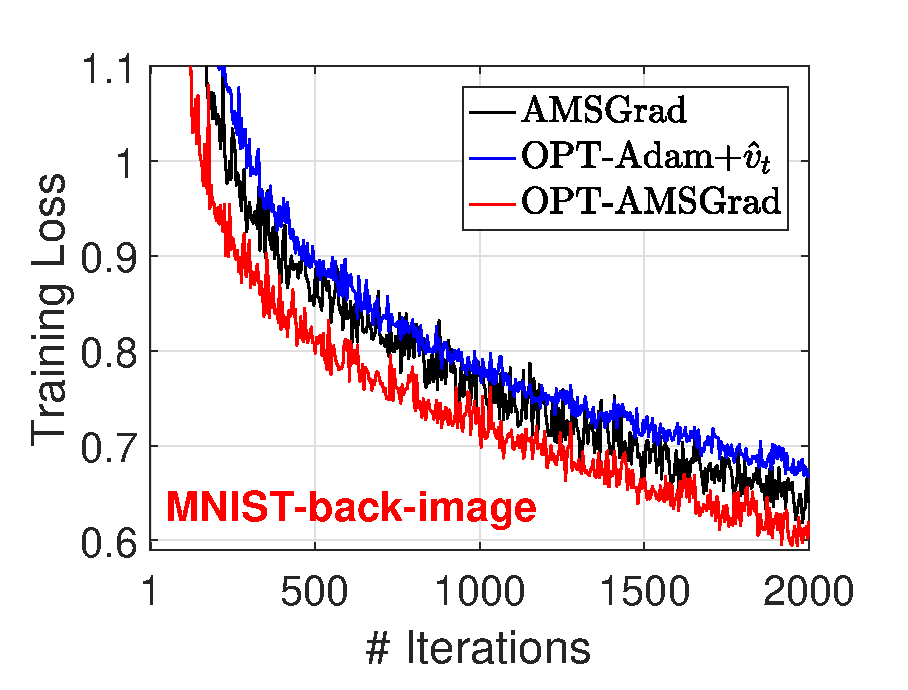
\includegraphics[width=1.8in]{simulation/fig2/M_image_train_loss_no1.eps}\hspace{-0.12in}
% \includegraphics[width=1.8in]{simulation/fig2/cifar_cnn_train_loss_no1.eps}
% }

% \mbox{\hspace{-0.2in}
% \includegraphics[width=1.8in]{simulation/fig2/imdb_lstm_train_loss_no1.eps}\hspace{-0.12in}
% \includegraphics[width=1.8in]{simulation/fig2/cifar10_resnet_train_loss.eps}\hspace{-0.12in}
% \includegraphics[width=1.8in]{simulation/fig2/cifar100_resnet_train_loss.eps}
% }
% \caption{Training loss vs. Number of iterations for fully connected NN, LSTM, CNN and ResNet.}
% \label{fig:train_loss}\vspace{-0.15in}
% \end{figure}



%-----------------------------------------------------------------------------
%\vspace{0.4cm}

\end{document} 
